
%%%%%%%%%%%%%%%%%%%%%%%%%%%%%%%%%%%%%%%%%%%%%%%%%%%%%%%%%%%%%%%%%%%%%%%%
%    INSTITUTE OF PHYSICS PUBLISHING                                   %
%                                                                      %
%   `Preparing an article for publication in an Institute of Physics   %
%    Publishing journal using LaTeX'                                   %
%                                                                      %
%    LaTeX source code `ioplau2e.tex' used to generate `author         %
%    guidelines', the documentation explaining and demonstrating use   %
%    of the Institute of Physics Publishing LaTeX preprint files       %
%    `iopart.cls, iopart12.clo and iopart10.clo'.                      %
%                                                                      %
%    `ioplau2e.tex' itself uses LaTeX with `iopart.cls'                %
%                                                                      %
%%%%%%%%%%%%%%%%%%%%%%%%%%%%%%%%%%
%
%
% First we have a character check
%
% ! exclamation mark    " double quote  
% # hash                ` opening quote (grave)
% & ampersand           ' closing quote (acute)
% $ dollar              % percent       
% ( open parenthesis    ) close paren.  
% - hyphen              = equals sign
% | vertical bar        ~ tilde         
% @ at sign             _ underscore
% { open curly brace    } close curly   
% [ open square         ] close square bracket
% + plus sign           ; semi-colon    
% * asterisk            : colon
% < open angle bracket  > close angle   
% , comma               . full stop
% ? question mark       / forward slash 
% \ backslash           ^ circumflex
%
% ABCDEFGHIJKLMNOPQRSTUVWXYZ 
% abcdefghijklmnopqrstuvwxyz 
% 1234567890
%
%%%%%%%%%%%%%%%%%%%%%%%%%%%%%%%%%%%%%%%%%%%%%%%%%%%%%%%%%%%%%%%%%%%
%
%%novalidate

\documentclass[12pt,a4paper,final]{iopart}
\newcommand{\gguide}{{\it Preparing graphics for IOP journals}}
%Uncomment next line if AMS fonts required
\expandafter\let\csname equation*\endcsname\relax
\expandafter\let\csname endequation*\endcsname\relax
\usepackage{amsmath}
\usepackage{iopams}  
\usepackage{graphicx}
\usepackage{biblatex}
\addbibresource{works.bib}
\usepackage[breaklinks=true,colorlinks=true,linkcolor=blue,urlcolor=blue,citecolor=blue]{hyperref}
% \usepackage{amsmath}
% \usepackage{setspace}
% \doublespacing

\begin{document}

\title[Neural response representation - IW Report]{Neuron population response representation in recurrent neural network models}

\author{Zach Cohen}
\address{Department of Computer Science}
\address{Princeton University}
\address{Princeton, NJ 08544}
\ead{zacohen@princeton.edu}

\author{\emph{Advised by}: Dr. Jonathan Pillow}
\address{Princeton Neuroscience Institute}
\address{Princeton University}
\address{Princeton, NJ 08544}
\ead{pillow@princeton.edu}

\begin{abstract}
The mechanism underlying the way in which the brain coordinates the integration of relevant and irrelevant sensory inputs based on a context has long eluded neuroscientists. In recent years, advances in cognitive modeling using artificial neural networks has allowed theoreticians to gain deeper insight into the neurological processes that give rise to complex behaviors. In this work, we present a cognitive model that does the task of encoding, representing, and decoding stimuli, and coordinating a response to such stimuli based on a context cue. We then decompose the model to understand how this process unfolds, treating the model as a high-dimensional, dynamical process. We consider past proposed mechanisms underlying context-dependent feature integration, and amend and extend previous theories for how this process occurs at the population level of neurons.
\end{abstract}

% %Uncomment for PACS numbers title message
% \pacs{00.00, 20.00, 42.10}
% % Keywords required only for MST, PB, PMB, PM, JOA, JOB? 
% \vspace{2pc}
% \noindent{\it Keywords}: Article preparation, IOP journals
% % Uncomment for Submitted to journal title message
% \submitto{\JPA}
% % Comment out if separate title page not required
% %\maketitle

\section{Introduction}
\label{sec:intro}
Our daily experiences are rich with sensory data. A vital task of the brain is to perceive, characterize, and respond to relevant sensory input while efficiently managing irrelevant sensory information, either by discarding it altogether, or gating it, in order to make an informed decision with respect to some goal state \cite{JDCohen:2001, Noudoost:2010}. For example, when a person is about to cross a street, he or she is presented with several streams of sensory information: the outside temperature, the visual information conveying the distance of oncoming cars from the cross-walk, the sound of an automated voice that instructs when it is safe to cross the street, and much more. Before crossing, this person must identify and attend to relevant streams of information (in this case, the visual information informing the distance of oncoming cars), while effectively shifting attention, either deliberately, or as is often the cause, automatically, away from sensory information that distracts from completing the task of crossing the street (in this case, the outside temperature). This task is as dynamic as it is essential: new streams of sensory information can appear unexpectedly (a voice of a friend pleading to wait until he/she catches up), and faltering in shifting attention dynamically to relevant streams of information can result in accidents and injuries (if one focuses too intently on the outside temperature, one might not be aware of a car barreling down the street).

More generally, the brain is responsible for encoding, processing and responding to sensory information with regard to an evolving internal representation of a contextual state in which the brain is operating or with respect to a goal state \cite{Desimon, JDCohen:2001}. Animals possess a remarkable ability to update internal representations of context and respond to similar or varying sensory stimuli in accordance with a set of context-dependent parameters \cite{Desimon}. A breadth of literature suggests that the neural basis for mediating a modulated response to varying sensory input based on a context resides primarily in prefrontal cortex (PFC) \cite{Desimon, Harvey, JDCohen:2001, Noudoost:2010, Tanji}, which plays a key role in executive functioning \cite{JDCohen:2001}, executive control \cite{Rossi}, and a wide range of abstract, high-level reasoning tasks \cite{Desimon, Drewe, Fletcher, Tanji}. The exact nature of this mechanism, how PFC accomplishes the vital task of shifting sensory attention based on context, remains poorly understood.

The goal of the theoretical neuroscientist is to respond to this dilemma. Rather than observe and record neural phenomena, the theoretical neuroscientist attempts to characterize and model them, using advanced computational techniques and mathematical tools, in order to gain deeper insight into the underlying mechanism mediating such phenomena, to \emph{describe} these phenomena, and how they occur, rather than simply taking note of them \cite{Abbott2008}. As has been demonstrated in the past $25$ years, which have seen the explosion of computational learning and modeling techniques, a great deal of insight can be earned by modeling neural phenomena using artificial, but biologically inspired, tools \cite{Abbott2008}. Such tools, while necessarily complicated, lend themselves naturally to deeper investigation: while decomposing a subject's brain and measuring with even the utmost precision the strength of each synapse between each neuron (a task that, on its own, would take hundreds, if not thousands, of years) may yield similar results, such methods are impractical. Decomposing the weight matrix of synaptic connections in, say, an artificial neural network, however, is quite easy.

Recurrent neural networks (RNNs), which possess biologically inspired recurrent connectivity and flexible learning capabilities, have served in recent years as exciting and rich potential models for neural dynamics and brain functioning \cite{Mante2013,Miconi,Rajan,BarakSussillo,Williams}, particularly in learning and executing complex tasks that require attending to and shifting between various streams of incoming information. RNNs exhibit dynamic and chaotic behavior, which has previously made them both difficult to train and even more difficult to analyze \cite{Abarbanel, Sussillo}. However, recent training techniques have been developed that broaden the array of tasks RNNs can effectively accomplish, and techniques for analyzing RNN functioning have been devised in parallel, allowing for stronger inferential claims to be made regarding biological neural dynamics based on RNN dynamics observed in learning and accomplishing biologically relevant tasks \cite{Sussillo}. Some of the most recent efforts aimed at uncovering the underlying mechanism for how PFC accomplishes complex, context-dependent tasks have been the result of training correlate RNNs to perform the same complex tasks, and performing analysis on the network as it learns and reproduces the target behavior \cite{Mante2013}.

The goal of this work is to extend previously used neural network models for PFC functioning with the hopes of making stronger claims about how PFC accomplishes the task of responding to sensory information within a contextual regime. To accomplish this goal, we will update an existing RNN model and test the model's ability to reproduce more biologically relevant tasks than have previously been considered. We will then follow the lead of past work, described below, in attempting to construct a semi-quantitative view of how the neural network accomplishes the task we train it to perform.

\section{Background and related work}
\label{sec:back}
Building and extending upon previous advances in neural network models \cite{Jaeger}, Sussillo and Abbott showed in 2009 that randomly initialized, strongly recurrently connected neural networks, while exhibiting chaotic and unstable behavior before training, could be trained to produce periodic and coherent patterns \cite{Sussillo}. The training technique developed by Sussillo and Abbott, called FORCE (First-order reduced and controlled error) is derived from a recursive least-squares filter (RLS). FORCE learning, described in greater detail later in the text, as Sussillo and Abbott showed, can be applied to a vector external to the generator network of an RNN that tracks only the weight of each neuron on the output of the network. It can also be applied directly to the connectivity matrix within the network (corresponding, in a biological sense, to the synaptic connection strength between neurons in a biological brain). 

In 2013, Barak and Sussillo attempted to open the black box concealing the mechanism of action for trained neural network models by studying the trained models as high-dimensional dynamical systems \cite{BarakSussillo}. After training, Barak and Sussillo argued, the network models possessed several fixed and slow points in the otherwise chaotic high-dimensional space induced by network activity. Barak and Sussillo found that by linearizing around fixed and slow points in the state space of a trained model (described in greater detail in \hyperref[sec:imp]{Implementation}), they could reproduce and better characterize the flexible, dynamic activity patterns exhibited by network models after being trained to produce certain tasks, particularly ones that called for varying behavior based on a context.

In a 2013 study that would take advantage of the partially opened black box of neural network model function, Mante et al., suggested a novel mechanism for PFC stimulus feature integration in context-dependent tasks \cite{Mante2013}. In their study, Mante et al. trained macaque monkeys to perform a context-dependent feature discrimination task, visualized in Appendix C. The monkeys were presented with a rendering of randomized dots on a display, which, in each trial, had some motion (drifting to the left or right) and color (primarily red or green) coherence. In each trial, the monkeys were presented with a context cue, instructing them to focus on and later report with a saccade either the color or motion coherence of the dots. During this task, neural recordings were taken from the frontal eye field (FEF), an area of PFC that manages saccadic eye movement. These recordings were taken at the population level of neurons in the FEF. When Mante et al. isolated principal components of the population-level neural firing rates, they found that PFC neural dynamics, like those in the network models in \cite{BarakSussillo} could be readily understood within the context of an evolving dynamical system (see Appendix C for more details).

In the feature selection and integration scheme described by Mante et al., incoming sensory evidence perturbs neural population firing rates along one of several ``choice axes'' in the state space represented by the population activity of recorded neurons (in the experiment outline above, there are two primary axes for color and motion contexts; the positive direction of each axis represents a choice corresponding to one of the two possible saccadic eye movement—left or right eye movement—and the negative direction represents the opposite choice) in the dynamical system. As evidence accumulates, the population firings rates are further and further perturbed along the corresponding choice axis until the monkey responds with a saccade; at which point the population recordings collapse on the corresponding choice point (the terminal point along the choice axis that is furthest along the axis from the starting point of the population firing rates). Notably, and importantly for the integration scheme that Mante et al. propose, the context in which the monkey was performing the task had little influence on the strength of the perturbation of the neural firing rates along the choice axes for either feature. In other words, whether or not the monkey was instructed to report color or motion coherence, the neural firing rate trajectories along the respective axes for color or motion were still robust and observable. In the end, the monkey was still able to discriminate relevant sensory data, despite neural recordings which suggested that the irrelevant sensory data was still being accumulated in PFC neurons.

This observation defied several prominent theories for how sensory data is accumulated in PFC in contextual regimes \cite{Mante2013}. Some key models for how PFC integrates streams of relevant and irrelevant data, like early selection models, suggest that PFC essentially “gates” downstream irrelevant sensory pathways (if the context dictates that the monkey should attend only to color data, the pathways between visual cortex and PFC responsible for encoding motion data are dampened or silenced entirely) \cite{JDCohen:2001}. Mante et al.'s findings, unlike previously suggested models, were counterintuitive: if PFC accumulates both relevant and irrelevant streams of data, how, in the end, is it able to properly discriminate between these streams?

To attempt to answer this question, Mante et al. trained a neural network model to perform the same task, and performed the same linearized dynamic analysis of the network that Barak and Sussillo had developed earlier. They found that the dynamics observed in PFC (the scheme in which sensory data induces perturbations along a choice axis towards a choice variable) were also observed in the neural network model. Further analysis of the network model uncovered a potential mechanism that could explain the results that Mante et al. observed in the PFC integration data: during the task, the neural network model (and, as Mante et al. extrapolate, PFC) maintains a selection vector that is context-dependent and that points along the relevant choice axis and orthogonal to the irrelevant choice axis. While relevant and irrelevant sensory data perturb the network model (and, analogously, neural population spikes) along both the relevant and irrelevant choice axes, the system essentially “relaxes” along the axis orthogonal to the selection vector (but not along the axis parallel to the selection vector), and so the network model ``ends up'' in the correct choice point after sufficient accumulation of evidence, even while relevant and irrelevant streams of information are incorporated into the dynamical process.

Mante et al. reasoned, after roughly replicating PFC dynamics in their neural network model, that the selection vector scheme observed in the network model was a plausible explanation for the observed PFC dynamics. Of course, this claim calls for a fair amount of refinement. Mante et al. make a strong claim about feature integration in PFC based on observations of a network model trained to complete an arbitrary task that involves feature integration. Mante et al.'s work acts as a more compelling explanation for how the network accomplishes the task itself, rather than as a feasible model for how PFC performs context-dependent evidence accumulation and computation.

With this study, we plan to make a necessary refinement to Mante et al.'s claims and contribute stronger claims about the nature of context-dependent feature integration in PFC to the larger literature. To accomplish this task, we train a network model similar to the one Mante et al. used, using the FORCE learning procedure, rather than backpropagation through time (BPTT), which Mante et al. used in their study, for reasons detailed below, to reproduce the neural data recorded from the task, rather than the feature discrimination task alone. This allows the inferential claims made about PFC feature integration to be more robust than those that Mante et al. made. Logically, this holds: to make stronger claims about PFC, we train our model to behave just like the object it is modeling (by outputting neural data, rather than an arbitrary task variable). We will also attempt to move away from the deterministic nature of the neural network model model used in Mante et al.’s study in order to increase the likeness of the network model model to how actual PFC functions (detailed more in methods). We then investigate the mechanism for how the model is learning and reproducing the neural data. Through these combined efforts, we hope to make stronger claim about the nature of PFC feature integration and provide a more advanced neural network model for future work investigating the nature of highly complex neural computations.

\section{Approach}
\label{sec:app}
For this report, we start with a randomly initialized, strongly recurrent neural network. We trained all networks with FORCE or full-FORCE (both detailed \hyperref[sec:imp]{Implementation}). We preferred procedures that employ some sort of weight filtering over BPTT, mainly because of the immensely high-dimensional nature of our ultimate target function. BPTT requires unrolling the RNN over long stretches of time, which becomes computationally expensive, particularly in networks similar in size to the ones we used. 

The key element distinguishing our work from past studies is the nature of our target function. We use a neural dataset provided by the study run by Mante et al., outlined in the previous section. We sorted the data based on ``conditions,'' or trials in which the color coherence value, motion coherence value, and context (what relevant stimulus the monkey was instructed to attend to) were the same, across ``units'' or individual files of neural recordings taken from the same site in monkey FEF. We smoothed the data to make it analyzable by our RNN, and then trained our model to reproduce varying neural data streams that were sorted based on context and provided evidence. We then tested the accuracy of our model in reproducing the target neural data in varying contexts, effectively testing the model's robustness to be used as a model for neural computation.

We finally decomposed our network model to attempt to reconstruct how it performed the task for integrating relevant versus irrelevant streams of information based on a context.

All network models and training procedures were written from scratch in Python, using the \texttt{numpy} and \texttt{scipy} packages. All plots were rendered using Matplotlib \cite{Hunter:2007}. We refrained from using pre-built models provided by tools like PyTorch and TensorFlow in order to retain maximum flexibility in implementation, and because these pre-built models often lack biological relevance and plausibility, which is ultimately what we were after in building these models. All code is available for view at: \hyperref[https://github.com/zachcohen1/recurrent]{\texttt{https://github.com/zachcohen1/recurrent}}

\section{Implementation}
\label{sec:imp}
\subsection{Network architecture}
For all experiments, we start with a randomly initialized, strongly recurrent neural network. The activities of neurons in the network are described by:
\begin{equation}
    \tau \dot{{\bf x}} = -{\bf x} + \boldsymbol{J}r({\bf x}) + \boldsymbol{J}^I{\bf b} + {\bf \epsilon}
\end{equation}

\begin{figure}
    \centering
    \includegraphics[width=\linewidth]{neuralnetworkZ.png}
    \caption{An illustrated schematic of the network model's structure. All units in the network are strongly, recurrently connected, and target functions are read out via a linear combination of weight that are learned during training. A final behavioral node integrates the neural output and reports a behavioral task variable (either reporting $+1$ or $-1$ depending on the coherence values of the relevant input stimuli).}
    \label{fig:my_label}
\end{figure}

where $\tau$ is a time constant, $x_i$ is the activity of neuron $i$, $\boldsymbol{J}$ is a recurrent weight matrix such that $J_{ij}$ describes the strength of connection between neurons $i$ and $j$, and $J_{ij} \sim \mathcal{N}(0, g^2/N)$, where $g$ is a hyperparamter, the magnitude of which determines the strength of connections between neurons in the network, and $N$ is the number of neurons in the network. At each timestep, the activity of the network from  the previous timestep is introduced to the network via a nonlinear function $r(\cdot)$; for all experiments, we used $r({\bf x}) = \tanh({\bf x})$. The input to neuron $i$ is determined by $(\boldsymbol{J}^I{\bf b})_i$, and $J^I_i \sim U([0, 1])$. Finally, ${\bf \epsilon}$ is a vector of stochastic noise introduced directly on to each neuron, and $\epsilon_i \sim \mathcal{N}(0, \sigma^2)$. For most experiments, we used $\sigma^2 \in [0, 1]$.

For each network simulation, we solved the above network equation over some time interval $\delta t$ using Euler integration:
\begin{align*}
    ({\bf x}(t+\delta t) - {\bf x}(t)) / \delta t &= -{\bf x}(t) + \boldsymbol{J}r({\bf x}(t)) + \boldsymbol{J}^I{\bf b} + {\bf \epsilon} \\
    {\bf x}(t+\delta t) - {\bf x}(t) &= \delta t(-{\bf x}(t) + \boldsymbol{J}r({\bf x}(t)) + \boldsymbol{J}^I{\bf b} + {\bf \epsilon}) \\
    {\bf x}(t+\delta t) &= (1 - \delta t){\bf x}(t) + \delta t \boldsymbol{J}r({\bf x}(t)) + \delta t \boldsymbol{J}^I{\bf b} + \delta t {\bf \epsilon}
\end{align*}
for time $t \in [0, T)$ for some predetermined time interval size $T$. The readout at each time-step is ${\bf w}r({\bf x}(t))$, ${\bf w}$ is a set of weights external to the network that are ``learned'', with respect to some target function, through various training procedures defined in the following subsections.

For modeling the output of both neural data and the target behavioral task variable, we define a final node in the network, which we denoted as $z$, that is virtually external, but still within the network. This node is defined as 
\[
    \tau \dot{z} = -z + {\bf w}r({\bf x})
\]
and is trivially solved, like above, as $z_{t + \delta t} = (1-\delta t) z(t) + \delta t {\bf w}r({\bf x}(t))$. Effectively, the behavioral node is a readout of weighted sum of the non-linear activations of the nodes in the network at each time step, but its dynamics are not explicitly reintroduced into the other nodes in the network at each time step. In other words, the behavioral node is ``aware'' of other nodes' readouts in the network, but other nodes are unaware of its state. 

In order to model context-dependent feature integration task outlined in \cite{Mante2013}, we used stimulus vectors ${\bf b} = \left(\mathsf{cc} \ \ \mathsf{mc} \ \ \mathsf{ac} \ \ \mathsf{am}\right)^T$, where $\mathsf{cc}, \ \mathsf{mc} \in \{-0.5, -0.17, -0.05, 0.05, 0.17, 0.5\}$, and $\mathsf{ac} = 1, \mathsf{am} = 0$ in the color context, and $\mathsf{ac} = 0, \mathsf{am} = 1$ in the motion context. The target behavior includes reporting the sign of the relevant stimulus. For example, if $\mathsf{am} = 1$, and $\mathsf{mc} = 0.5$, we would expect the network to report that it has integrated ``positive'' motion coherence, by reporting $z = 1$

We use this model structure for several reasons. Principally, this model has very few ``built-in'' features, which allows it to act as a general model of population-level neural computation, or else, the network is not designed for any one specific task, and thus, like the brain, is able to perform a wide range of tasks that are mutually unrelated. Ultimately, we are looking to deduce the underlying structure of how context-dependent information is represented in the brain: the recurrent weights of the RNN simulate recurrent connectivity between neurons in the biological brain, allowing neurons in one area of the network to communicate with other ones, particularly over time.

\subsection{FORCE learning}
The FORCE \cite{Sussillo} training technique minimizes the following cost function with respect to some target function $f(t)$:
\begin{equation*}
    \mathcal{C} = \frac{1}{T} \sum_{t = 1}^T \lVert r({\bf x}(t)){\bf w} - f(t) \rVert^2
\end{equation*}

The FORCE algorithm accomplishes this by learning weights on ${\bf w}$ using the RLS filter (detailed in Appendix A). The filter seeks to elect weights ${\bf w}$ that minimize $\mathcal{C}$, which is done by first calculating the error signal $e(t)$ between desired output $f(t)$ and network output $r({\bf x}(t)){\bf w}(t - \delta t)$,
\[
    e(t) = r({\bf x}(t)){\bf w}(t - \delta t) - f(t)
\]
and using the calculated error signal $e(t)$ to update the weights at each iteration ${\bf w}(t)$,
\[
    {\bf w}(t) = {\bf w}(t - \delta t) + e(t)\boldsymbol{P}(t)r({\bf x}(t))
\]
and then finally, updating the cross-correlation matrix $\boldsymbol{P}(t)$,
\[
    \boldsymbol{P}(t) = \boldsymbol{P}(t - \delta t) - \frac{\boldsymbol{P}(t-\delta t)r({\bf x}(t)) r({\bf x}(t))^T \boldsymbol{P}(t-\delta t)}{1 + r({\bf x}(t))^T\boldsymbol{P}(t-\delta t)r({\bf x}(t))}
\]
For the experiments detailed below, we employed a variant of the FORCE learning scheme that also adjusts weights of the connectivity matrix $\boldsymbol{J}$:
\[
    \boldsymbol{J}(t) = \boldsymbol{J}(t - \delta t) + \frac{e(t)\boldsymbol{P}(t)r({\bf x})}{1 + r({\bf x}(t))^T\boldsymbol{P}(t)r({\bf x}(t))}
\]
For these experiments, $\boldsymbol{P}(0) = \frac{1}{\alpha} \boldsymbol{I}$, where $\alpha$ is considered the approximate learning rate of the FORCE procedure (we typically used an $\alpha \ll N$, the number of neurons in the network, usually using $\alpha = 1$). Additionally, ${\bf w}(0) = \boldsymbol{0}$. 

With the above update rules, we can reason about how FORCE learning keeps the error signal re-introduced into the network from its output small. Because we initialize ${\bf w}(0) = \boldsymbol{0}$, we can rewrite $e(\delta t)$ (the error signal after the first step of FORCE) as:
\[
    e(\delta t) = \frac{-\alpha f(\delta t)}{\alpha + r({\bf x}(\delta t))^T r({\bf x}(\delta t))}
\]
Note that, at each time step, $r({\bf x})$ is a column vector composed only of entries $\in [-1, 1]$. Because each entry of ${\bf x}$ is initially drawn from a standard normal distribution, we can assume that a significant portion of the elements of $r({\bf x})$ will be of magnitude $1$ in the first time step, and, along that reasoning, that $r({\bf x}(\delta t))^T r({\bf x}(\delta t))$ will be of order $N$. As long as $\alpha \ll N_G$, we can reason that the first error term will take a value much less than 1 (unless $f(t) \gg N$, which, for all experiments presented in this paper, is not the case). Because the first readout error is small, the equations above imply that the following error term will be approximately equal to the target function, and that each successive error term will be therefore relatively small in relation to the activities of the neurons in the network. 

This fact is important for reasons: (1) such an error control allows for fast convergence over the filter weights ${\bf w}$ and recurrent weights $\boldsymbol{J}$, which is important when approximating high-dimensional target functions that carry with them high computational costs in modeling, and (2) because the error signal re-introduced to the network does not induce chaotic behavior in the RNN, which is often a challenge one must surmount in training RNNs to perform complex, temporally-dependent tasks.

The FORCE training procedure is described in greater detail in \cite{Sussillo}.

\subsection{full-FORCE learning}
The full-FORCE training scheme is a derived from FORCE learning \cite{DePasquale}. Where FORCE is derived with liquid and echo-state networks in mind, which focus primarily on minimizing a cost function with respect to the target function representation external to the network, i.e., by training weights external to the network, full-FORCE trains RNNs based on internal representation of target functions. full-FORCE learning trains an RNN using two different networks: a target-producing network and a task-performing network. The target-producing network is used only during training, and is not modified during the training procedure; rather it acts as a base network on which the synaptic weights of the task-performing network are trained.

The activities of neurons in the target-generating network are described by:
\[
    \tau \dot{{\bf x}}^D = -{\bf x}^D + \boldsymbol{J}^D r({\bf x}^D) + {\bf u}f(t) + {\bf u}_i f_i(t) + {\bf \epsilon}
\]
where the superscript $(\cdot)^D$ denotes a network feature of the target-generating network, ${\bf u}$ is a vector of weights on the function output by the task-performing network during training, $f(t)$, and ${\bf u}_i$ is a vector of weights on the input parameters, $f_i(t)$, input into both the target and task-performing networks, typically to denote some state or evidence for the network to integrate.

Again, the network equation for the target-generating network is solved over some time interval $\delta t$ using Euler integration:
\[
    {\bf x}^D(t + \delta t) = (1 - \delta t) {\bf x}^D(t) + \delta t \boldsymbol{J}^D r({\bf x}^D(t)) + \delta t {\bf u}f(t) + \delta t {\bf u}_i f_i(t) + \delta t {\bf \epsilon}
\]
and the network equation for the trained network is solved in the same way as the FORCE-trained network.

The goal of full-FORCE learning is to minimize the cost function:
\[
    \mathcal{C} = \frac{1}{T} \sum_{t=0}^T \lVert \boldsymbol{J} r({\bf x}(t)) - \boldsymbol{J}^D r({\bf x}^D(t)) - {\bf u}f(t) \rVert ^2
\]
where, here, $\boldsymbol{J}$ and $r({\bf x}(t))$ refer to the weight matrix and non-linear activations of the task-producing network, respectively. 

The training procedure proceeds more or less the same as that used for FORCE training, in which the RLS algorithm is run to minimize $\mathcal{C}$, the only differences being the calculation for $e(t)$, which becomes:
\[
    e(t) = \boldsymbol{J}(t - \delta t) r({\bf x}(t)) - \boldsymbol{J}^D r({\bf x}(t))^D - {\bf u}f(t)
\]
and the weight matrix update, $\boldsymbol{J}(t)$, which is:
\[
    \boldsymbol{J}(t) = \boldsymbol{J}(t - \delta t) - e(t)^T \boldsymbol{P}(t) r({\bf x}(t))
\]
where $\boldsymbol{P}(\cdot)$ is calculated in same way as FORCE, using the non-linear activations from the task-performing network. The details of full-FORCE are more fully developed in \cite{DePasquale}.

\subsection{Fixed-point analysis}
After training the network model to reproduce neural data and simultaneously complete the context-dependent feature integration task, we employed an approach delineated in \cite{BarakSussillo} to paint a quasi-quantitative picture of how the RNN completes the task.

\subsubsection{Locating local and global minima}
We rewrite equation (1) in compact notation: $\dot{\bf{x}} = F(\bf{x})$, where $F(\bf{x})$ is the right-hand side of equation (1). In order to understand the linear dynamics of the system represented by $\dot{\bf{x}} = F(\bf{x})$, we want to find areas in which dynamics are approximately linear, or where small perturbations around some point approximate linear activity, for reasons demonstrated in the following subsection.

To find fixed points in the system, we define an auxiliary, scalar function $q({\bf x}) = \frac{1}{2} \lVert F({\bf x}) \rVert^2$, which roughly corresponds to the squared speed of the system, divided by two, or the kinetic energy of the system around some point ${\bf x}$, and minimize it. We do this because, as a sum of squares, this function reaches its minimum where $F({\bf x})$ reaches its minimum, and it is a scalar function, and is thus amenable to optimization software for solving.

\subsubsection{Local linear dynamics}
Consider the Taylor expansion of $\dot{\bf{x}} = F(\bf{x})$ around some fixed point $\bf{x}$:
\[
    F({\bf x} + \delta {\bf x}) = F({\bf x}) + F'({\bf x})\delta {\bf x} + \frac{1}{2} \delta {\bf x}^T F''({\bf x}) \delta {\bf x} + \dots
\]
Because the point $\bf{x}$ is a fixed point, $F({\bf x}) = {\bf 0}$, and the second order term of the Taylor series (and all terms succeeding it) are approximately ${\bf 0}$, so the magnitude of first order term dominates all other terms, or else $\lVert F'({\bf x})\delta {\bf x} \rVert > \lVert F({\bf x}) \rVert$ and $\lVert F'({\bf x})\delta {\bf x} \rVert \gg \lVert \frac{1}{2} \delta {\bf x}^T F''({\bf x}) \delta {\bf x} \rVert$ (we are concerned primarily with perturbations $\delta {\bf x}$ that are quite small, which substantially reduce the magnitude of the $F''({\bf x})$ term). These inequalities illustrate why some points ${\bf x}$ such that $F({\bf x}) = {\bf 0}$ are ideal candidates for linearization: they afford us a lower bound on $\lVert \delta {\bf x} \rVert$, which is 0. In other words, all infinitesimally small perturbations $\lVert \delta {\bf x} \rVert > 0 $ around some points ${\bf x}$ such that $F({\bf x}) = {\bf 0}$ will generate local linear or approximately linear dynamics.

Because we examine dynamics around fixed points, or points where $F({\bf x}) = {\bf 0}$, our expansion of $F({\bf x} + \delta {\bf x})$ reduces to:
\[
    F({\bf x} + \delta {\bf x}) = F'({\bf x})\delta {\bf x} + \frac{1}{2} \delta {\bf x}^T F''({\bf x}) \delta {\bf x} + \dots
\]
let $\boldsymbol{p} = \delta {\bf x}$. Heeding the second inequality ($\lVert F'({\bf x})\delta {\bf x} \rVert \gg \lVert \frac{1}{2} \delta {\bf x}^T F''({\bf x}) \delta {\bf x} \rVert$), we omit the second order term of this expansion, which yields:
\[
    F({\bf x} + \boldsymbol{p}) = F'({\bf x})\boldsymbol{p} 
\]
which is the general form for a linear dynamical system: $\dot{\boldsymbol{p}} = F'({\bf x})\boldsymbol{p}$, which is linear in $\boldsymbol{p}$. Thus, when studying local linear dynamics around some fixed point ${\bf x}$, our analysis will primarily be concerned with the matrix $\boldsymbol{M} = F'({\bf x})$, the Jacobian of $F(\cdot)$. In fact, we can think of $\boldsymbol{M}$ as the approximation of the network around fixed points, which aids in the following analysis.

Because we're interested in understanding local linear dynamics around $\boldsymbol{M}$, we perform an eigendecomposition on $\boldsymbol{M}$:
\[
    \boldsymbol{M} = \boldsymbol{L} \boldsymbol{\Lambda} \boldsymbol{R}
\]
where the $i$-th row of $\boldsymbol{L}$ is the $i$-th left eigenvector of $M$, the $i$-th column of $\boldsymbol{R}$ is the $i$-th right eigenvector, and $\boldsymbol{\Lambda}$ is a diagonal matrix such that $\boldsymbol{\Lambda}_{ii}$ is the $i$-th eigenvalue corresponding to the $i$-th eigenvectors of $\boldsymbol{L}$ and $\boldsymbol{R}$.

We generate the left and right eigenvectors, namely because the localized linear system is diagonalized over the left eigenbasis, or else, each mode of the dynamical system evolves independently of the other ones. The independent evolution of modes in the left eigenbasis allows for a simplified analysis of the modes over time, as the dynamics along each axis spanned by the left eigenbasis can be studied in isolation of the evolution of other modes. The right eigenbasis gives us a transformation back to the basis spanned by $\boldsymbol{M}$ once we've transformed some vector space into the left eigenbasis, which allows us to study independent modes in the left eigenbasis, and then reorient them into the system described properly by $\boldsymbol{M}$.

Dynamical systems can operate in four ways in locally linear regimes. Let $\lambda$ denote an eigenvalue in $\boldsymbol{\Lambda}$. If $\mathsf{Re}(\lambda) > 0$, the system expands as it evolves in time along the axis spanned by the corresponding left eigenvector, if $\mathsf{Re}(\lambda) < 0$, the system contracts over time along the axis spanned by the corresponding left eigenvector, if $\mathsf{Im}(\lambda) \neq 0$, the system oscillates over time along the axis spanned by the corresponding left eigenvector, and if $\mathsf{Re}(\lambda) = 0$, the system integrates over time along the axis spanned by the corresponding left eigenvector. 

This follows from the solution to a linear dynamical system $\dot{\boldsymbol{p}} = F'({\bf x})\boldsymbol{p}$ where $\boldsymbol{M} = \boldsymbol{L} \boldsymbol{\Lambda} \boldsymbol{R}$:
\[
    {\bf x}(t) = \sum_{k = 0}^n ({\bf l}_k {\bf x}_0) {\bf r}_k e^{\lambda_k t} = \sum_{k = 0}^n ({\bf l}_k {\bf x}_0) {\bf r}_k e^{\mathsf{Re}(\lambda_k)}(\cos(\mathsf{Im}(\lambda_k) t)) + i \sin(\mathsf{Im}(\lambda_k) t)))
\]
where ${\bf r}_k$ is the $k$-th right eigenvector and ${\bf l}_k$ is the $k$-th left eigenvector.

Because we are interested in locally linear and stable regimes, and because we are interested in how incoming sensory evidence is incorporated and represented in the state space of our model, we follow the lead of Mante et. al. in \cite{Mante2013} and single out right and left eigenvectors corresponding to eigenvalues such that $\mathsf{Re}(\lambda) = 0$, or else where the above expression reduces to ${\bf x}(t) = \sum_{k = 0}^n ({\bf l}_k {\bf x}_0) {\bf r}_k e^{0 t} = {\bf x}(t) = \sum_{k = 0}^n ({\bf l}_k {\bf x}_0) {\bf r}_k$, such that the evolution of the system along the appropriated axes spanned by the left and right eigenvectors is fixed through time.

This scheme, as proposed in \cite{Mante2013}, affords us a simple mechanism for understanding how relevant stimuli are incorporated into the network. Along axes spanned by the left and right eigenvectors such that $\mathsf{Re}(\lambda) = 0$, the dynamics of the network are loosely understood as the magnitude of the projection of the stimulus vector onto left eigenvector that determines the extent to which a stimulus will be incorporated into the system. Thus, the orthogonal right and left vectors such that $\mathsf{Re}(\lambda) = 0$ provide approximate axes within the state space to approximate selective integration of sensory stimuli depending on a context.

\section{Data}
\label{sec:data}
Our target neural data set comes from Mante et al.'s study, and is comprised of neural recordings taken from FEF of two macaque monkeys trained to perform the context-dependent feature discrimination task described in \hyperref[sec:back]{Background and Related Work} and Appendix D. We followed Mante and Sussillo's procedure for parsing, cleaning and organizing the data, which we describe briefly in this section.

For their experiments, Mante et al. taught the task to two macaque monkeys, labeled A and F, and performed several, randomized trials in each recording session with both A and F. Each recording session is contained within its own \texttt{.mat} file; each one contains, on average, 1,200 trials for each unit. Each trial is comprised of a neural recording, lasting 850 ms, and values indicating the motion coherence of the dots on the display, the color coherence of the dots, the context of the trial (what feature the monkey was instructed to attend to), and whether or not the monkey correctly completed the trial by directing a saccade to the target.

The neural recordings from the experiments take the form of a sequence of 0's and 1's, one in each time bin. In each bin, 1 indicates detected electrophysiological activity, and 0 indicates the absence of any detected activity. Mante et al. performed their recordings with the hopes of analyzing neural behavior at the neuron population level; while this method allows for the analysis of neural dynamics across larger neural landscapes and greater insight into how populations of neurons act during activities of interest, this method of recording is also far less precise than single-neuron recordings. This results in remarkably high variability in the recorded neural response across trials in a single unit for which the monkey was presented the exact same information. This fact, along with the underlying assumption in our RNN model that functions it is trained to reproduce are continuous (unlike the binary nature of the neural recordings) requires us to manipulate the neural data in a way that preserves its structure but that also makes it more amenable to reproduction by our model. 

For each unit, we averaged the neural recordings across conditions. We identified 72 possible conditions for the data: some permutation of 6 possible motion coherence values and 6 possible color coherence values, and 2 possible contexts (attend to color coherence or attend to motion coherence). The experimental data for each unit had roughly the same number of trails for each of these conditions, which made averaging across them a reasonable estimate for neural activity in that unit in any particular condition. For each time bin in each condition, we calculated the average strength of the neural pulse by summing the neural activations across each time bin for each condition and divided by the number of trails in each respective condition. The neural data was collected at a frequency of 20 Hz; in order to minimize variability across bins, we resampled using a moving box filter that was the width of 20 bins. We then resampled again through time using a Fourier method.

Averaging across conditions for each unit and resampling allowed the data to more readily resemble the continuous, smooth functions that we wanted. The final step in preparing the data for replication was filtering it using a Gaussian kernel ($\sigma = 40$ ms, window width = $50$ ms). After smoothing, we reshaped the data, by z-scoring the value in each time bin and throughout each condition by subtracting the mean of the total average activity over the entire unit, and dividing by the standard deviation of the activity over the entire unit.

\section{Results}
\label{sec:res}

\subsection{Reproducing neural data}
We found that all networks used in this paper, regardless of training method, were able to successfully reproduce context-dependent neural data traces, dynamically changing output behavior to match target neural behavior, depending on input. In order to quantify how well the network model was able to reproduce neural data traces, we employed a statistic from \cite{Rajan}, $\mathsf{pVar}$:
\[
    \mathsf{pVar}_k = 1 - \frac{\Big(\sum_{i = 1}^N \sum_{t = 0}^T D_i^k(t) - r_i^k(t)\Big)^2}{\Big(\sum_{i = 1}^N \sum_{t = 0}^T D_i^k(t) - \bar{D}^k(t)\Big)^2}
\]
where $k$ is some condition.
\begin{figure}[t]
 \centering
 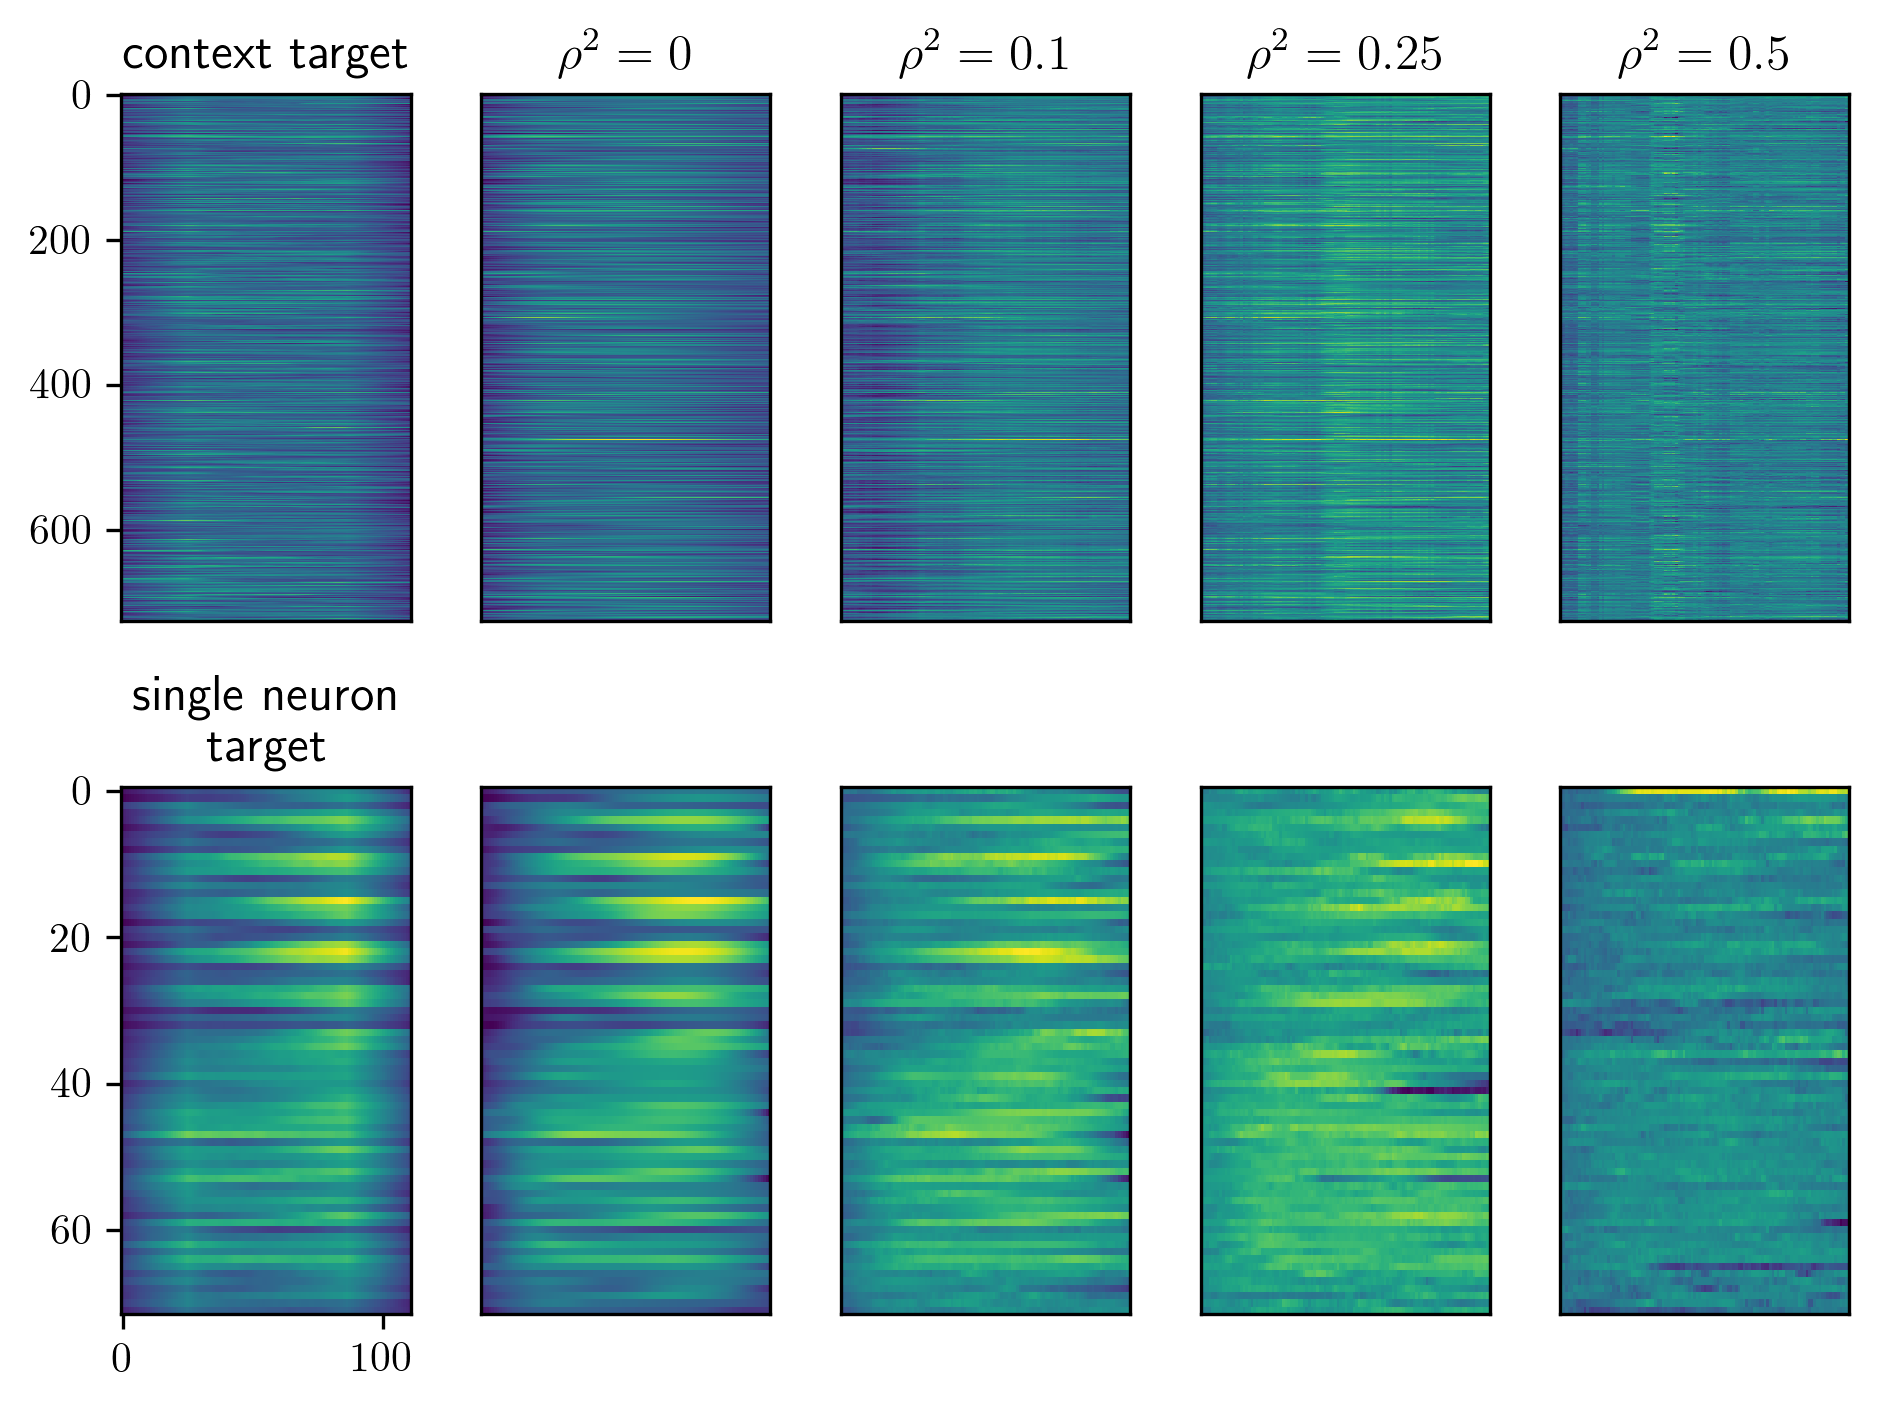
\includegraphics[width=\linewidth]{context_neuron_1_18.png}
 \caption{The results of a network trained with FORCE reproducing neural data traces, both in a deterministic setting, and with stochastic noise injected onto the stimuli input into the network. The top row shows the entire network's response to a single stimulus vector (strong, negative color coherence combined with strong, negative motion coherence, in the color context), and the second row shows a single neuron recorded over all $72$ possible stimulus/context combinations.}
\end{figure}
\begin{figure}[t]
 \centering
 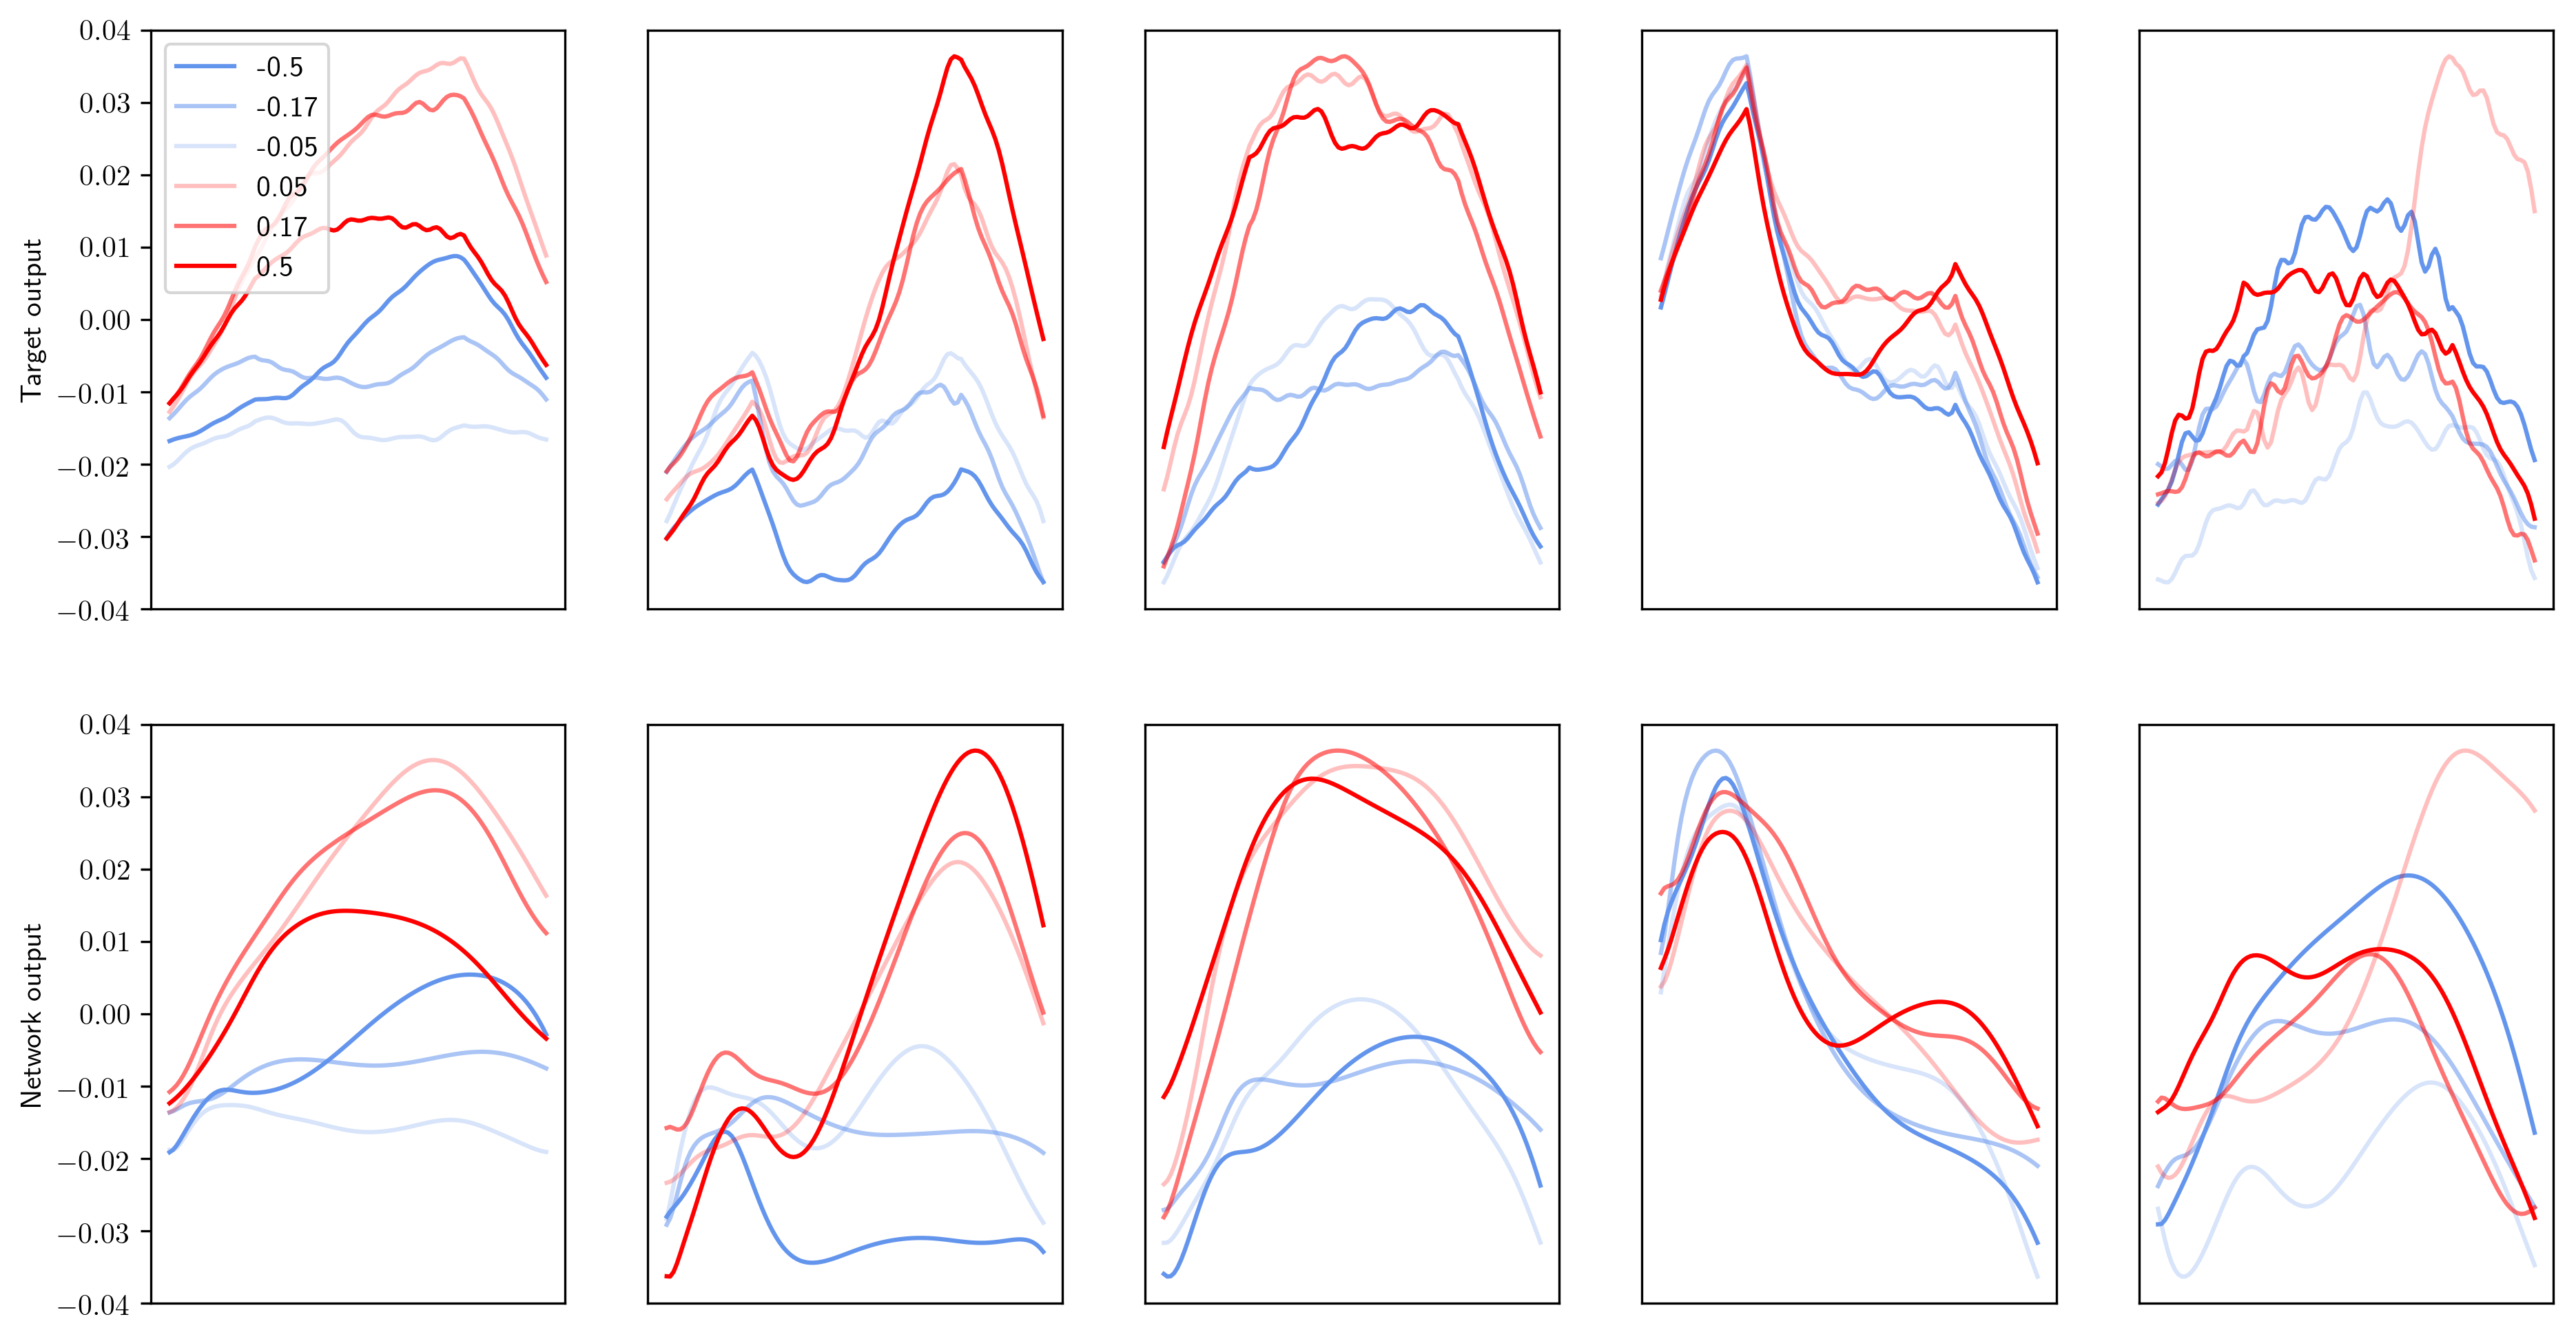
\includegraphics[width=\linewidth]{nc2_rho_0.png}
 \caption{The results of a network trained with FORCE reproducing neural data traces, aligned with the target behavior. The plots are organized by ``neuron." In the target data traces, this corresponds to the readout of a single electrode parsing population level responses, and in the network, this corresponds to one node in the network. Neurons in this trace were selected based on the clarity of the shifting response over time according to stimuli. In this figure, no noise is injected onto the stimuli.}
\end{figure}
\begin{figure}[h!]
 \centering
 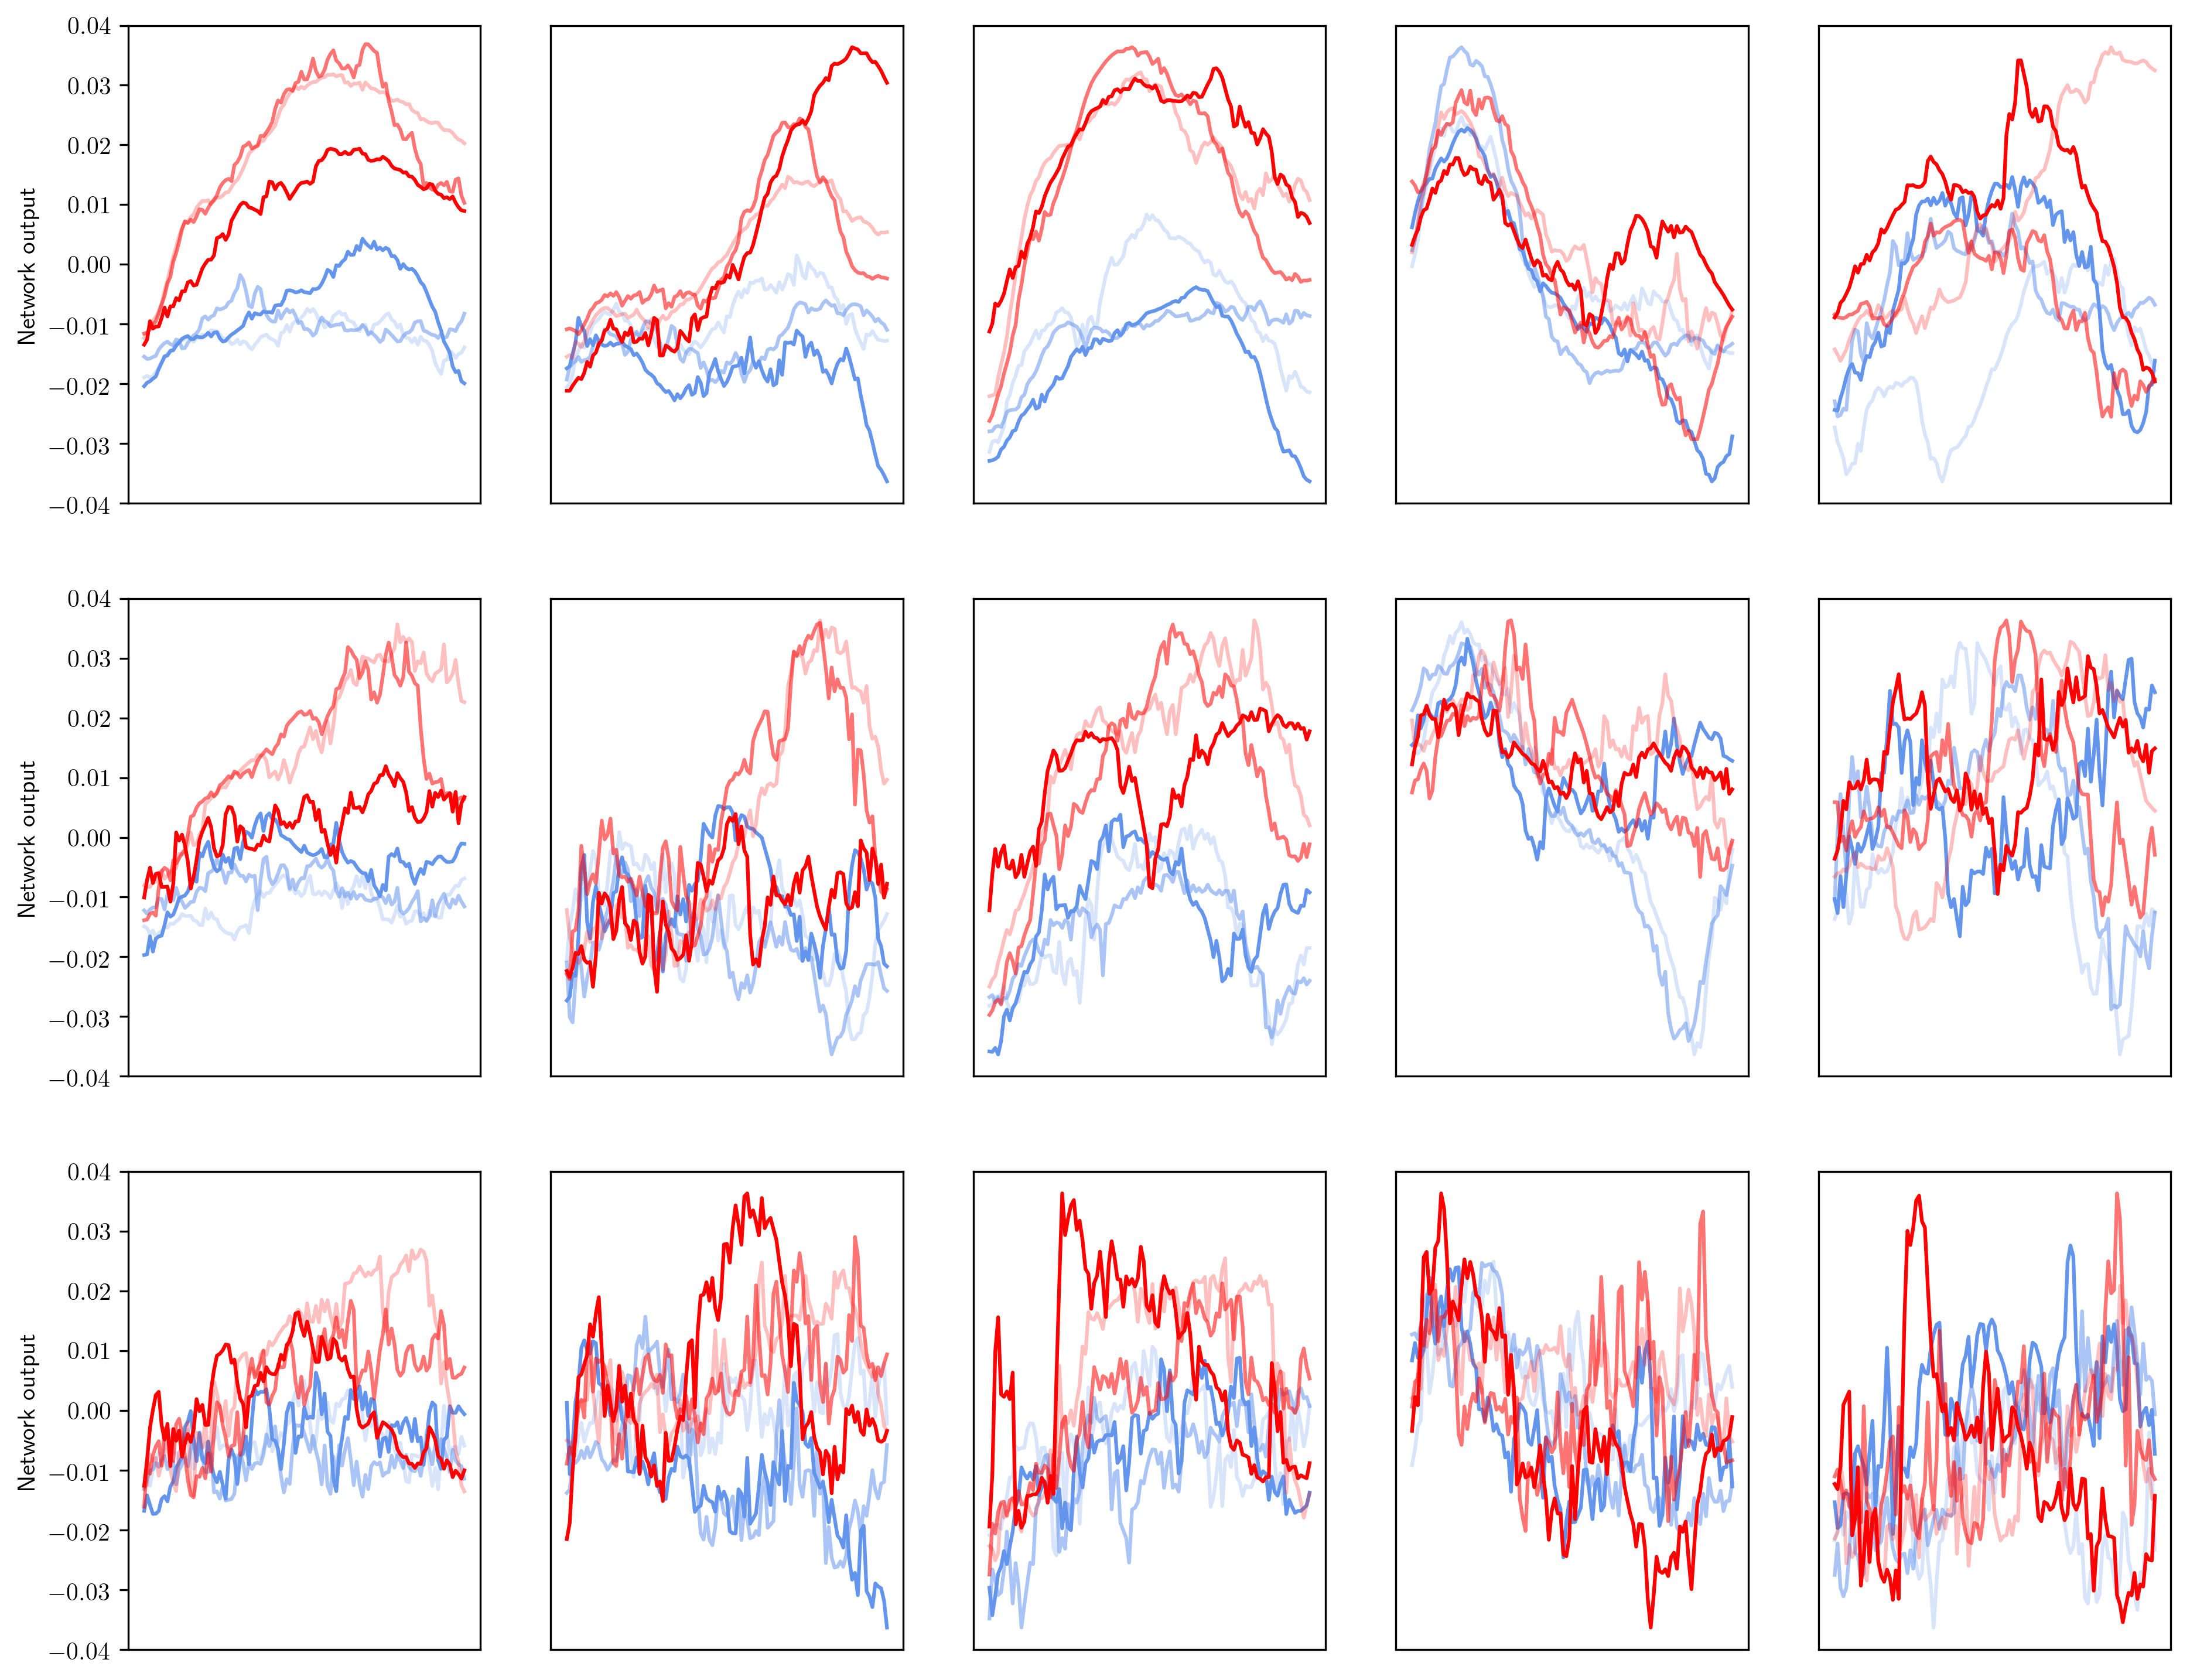
\includegraphics[width=\linewidth]{nc2_noise_comp.png}
 \caption{In this figure, the top row of plots is the network output when the input stimulus is corrupted by Gaussian noise with variance $\rho^2 = 0.1$; the second row with  $\rho^2 = 0.25$ and the third row with $\rho^2 = 0.5$. The target traces for each neuron are the same as in \emph{Figure 3}.}
\end{figure}

We tested the network in both a deterministic setting, and an induced stochastic setting. In order the achieve the latter, we injected stochastic noise into both the color and motion stimuli on both attend-motion and attend-color trials, and analyzed the output of the network. The full neural traces are displayed graphically in \emph{Figure 2}, showing the difference in response according to the varying strength of the noise injected onto the stimulus. Once again, in figure \emph{Figure 3-4}, we zoom in on singular neuron traces to get a more fine-grained view of how the network responds to various changes in noise injected onto the stimulus.

\subsection{Decoding neural data to generate encoded behavioral response}
Inspired by the flexibility of our model, we trained RNNs with FORCE learning to decode neural data traces and generate the target behavior (reporting positive/negative depending on color/motion coherence and context). Because neural firing patterns in the brain are typically noisy, we also injected stochastic noise into the neural data traces, as the network models attempted to decode them. We found that in the deterministic setting, the network was able to decode the neural data traces with ease, as demonstrated in \emph{Figure 5}, in the left panel. The accuracy of the decoding scheme began to degenerate as the magnitude of the stochastic noise began to increase.

For experiments involving generation of target \emph{behavioral} variables, we refrain from using explicit numerical measurements of error, and instead assign the score of ``correct" ($+1$) of ``incorrect" ($0$) in the event that the network successfully or unsuccessfully reproduces the target behavior based on the incoming neural trace, respectively. We found that the percent correct reported behavioral responses was quite similar to that of networks with an integrator node embedded within the network, summarized by \emph{Figure 7}.
\begin{figure}
    \centering
    \begin{minipage}{0.495\linewidth}
        \centering
        \includegraphics[width=\linewidth]{decoder_w_entire_network.png}
    \end{minipage}
    \begin{minipage}{0.495\linewidth}
        \centering
        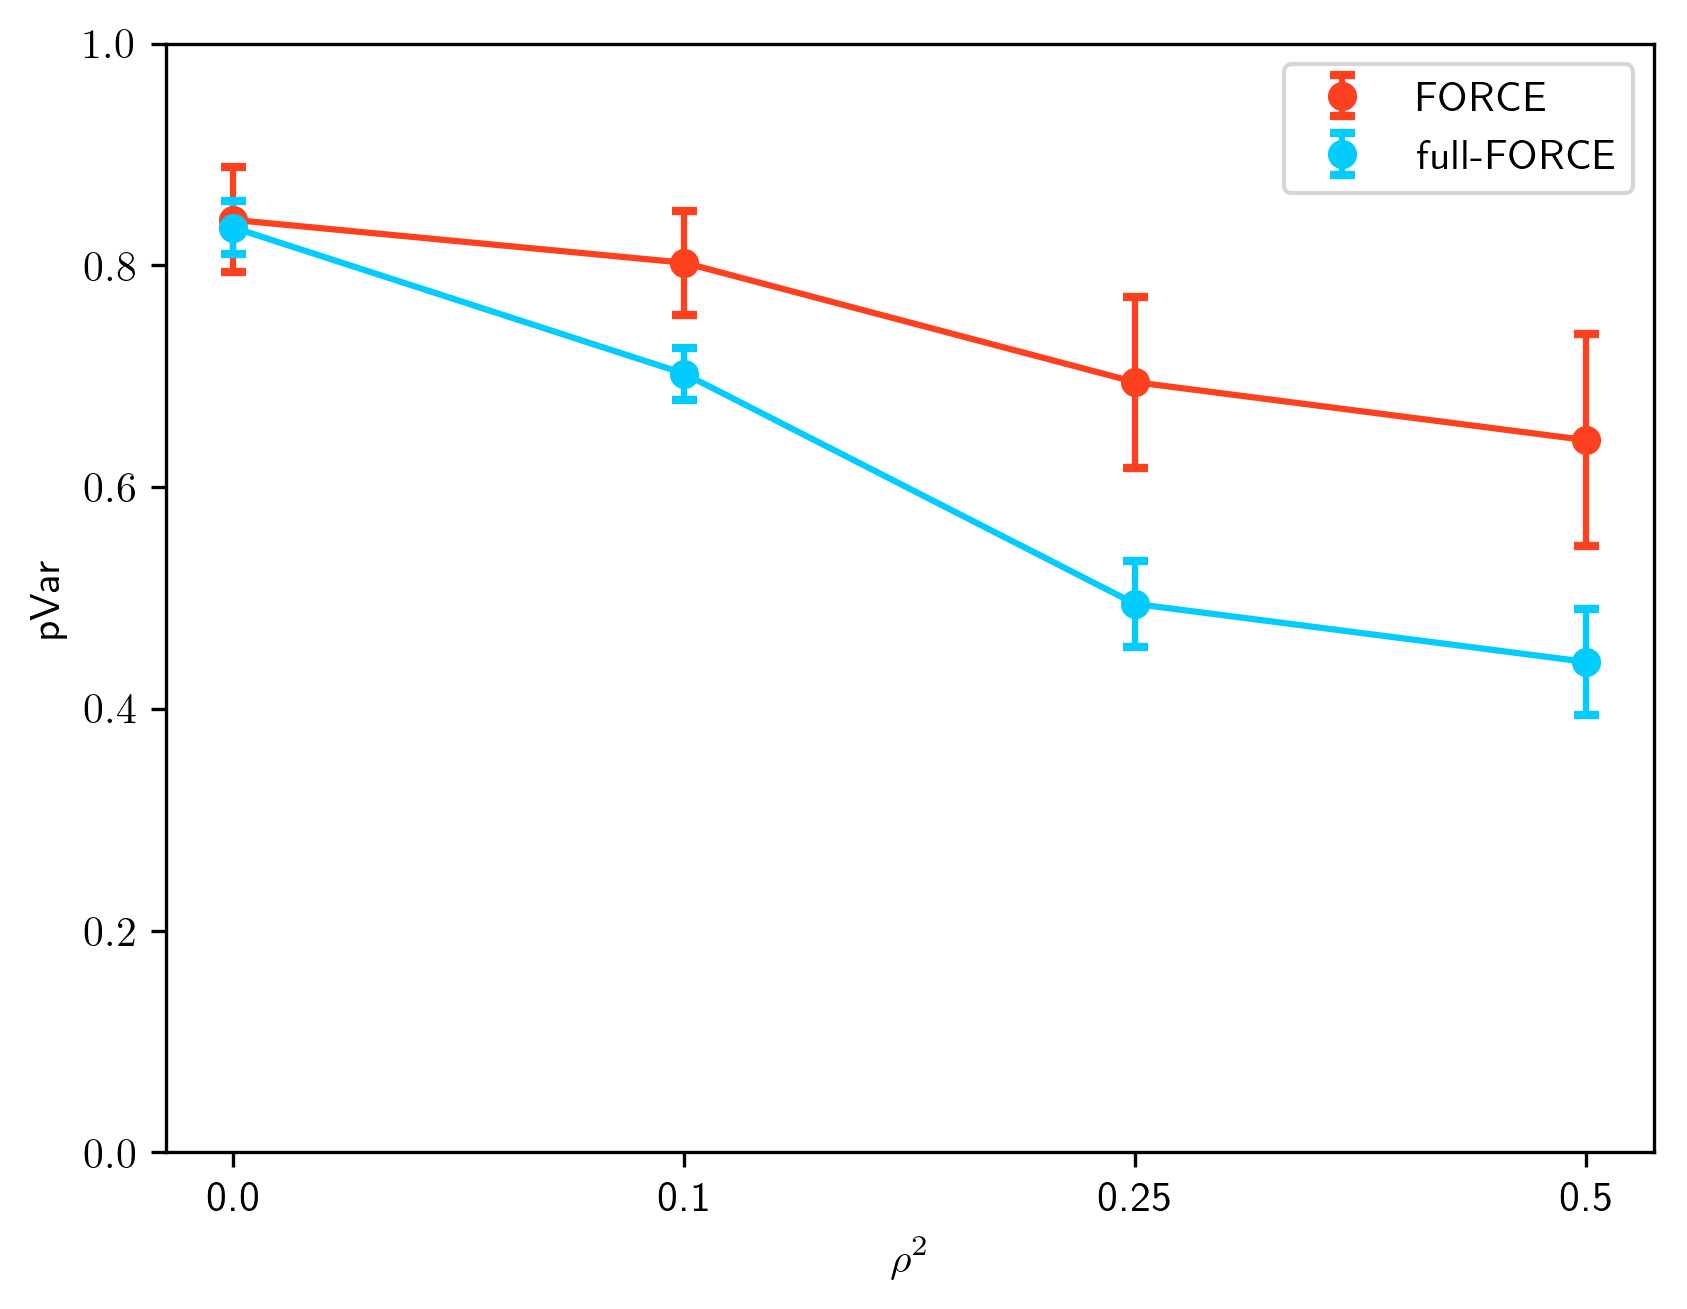
\includegraphics[width=\linewidth]{pvar_noise.png}
    \end{minipage}
    \caption{The left panel is a demonstration of the output of a network designed to decode neural data traces into target behavioral task variables. The right panel plots the $\mathsf{pVar}$ statistic, across different magnitudes stimulus noise.}
    \label{fig:my_label}
\end{figure}

\subsection{Generating behavioral response within the network}
In addition to training network models to decode the neural data traces, as fed into them from an external source, we also trained models to reproduce the target neural data traces in addition to generating the target behavior. 
\begin{figure}
    \centering
    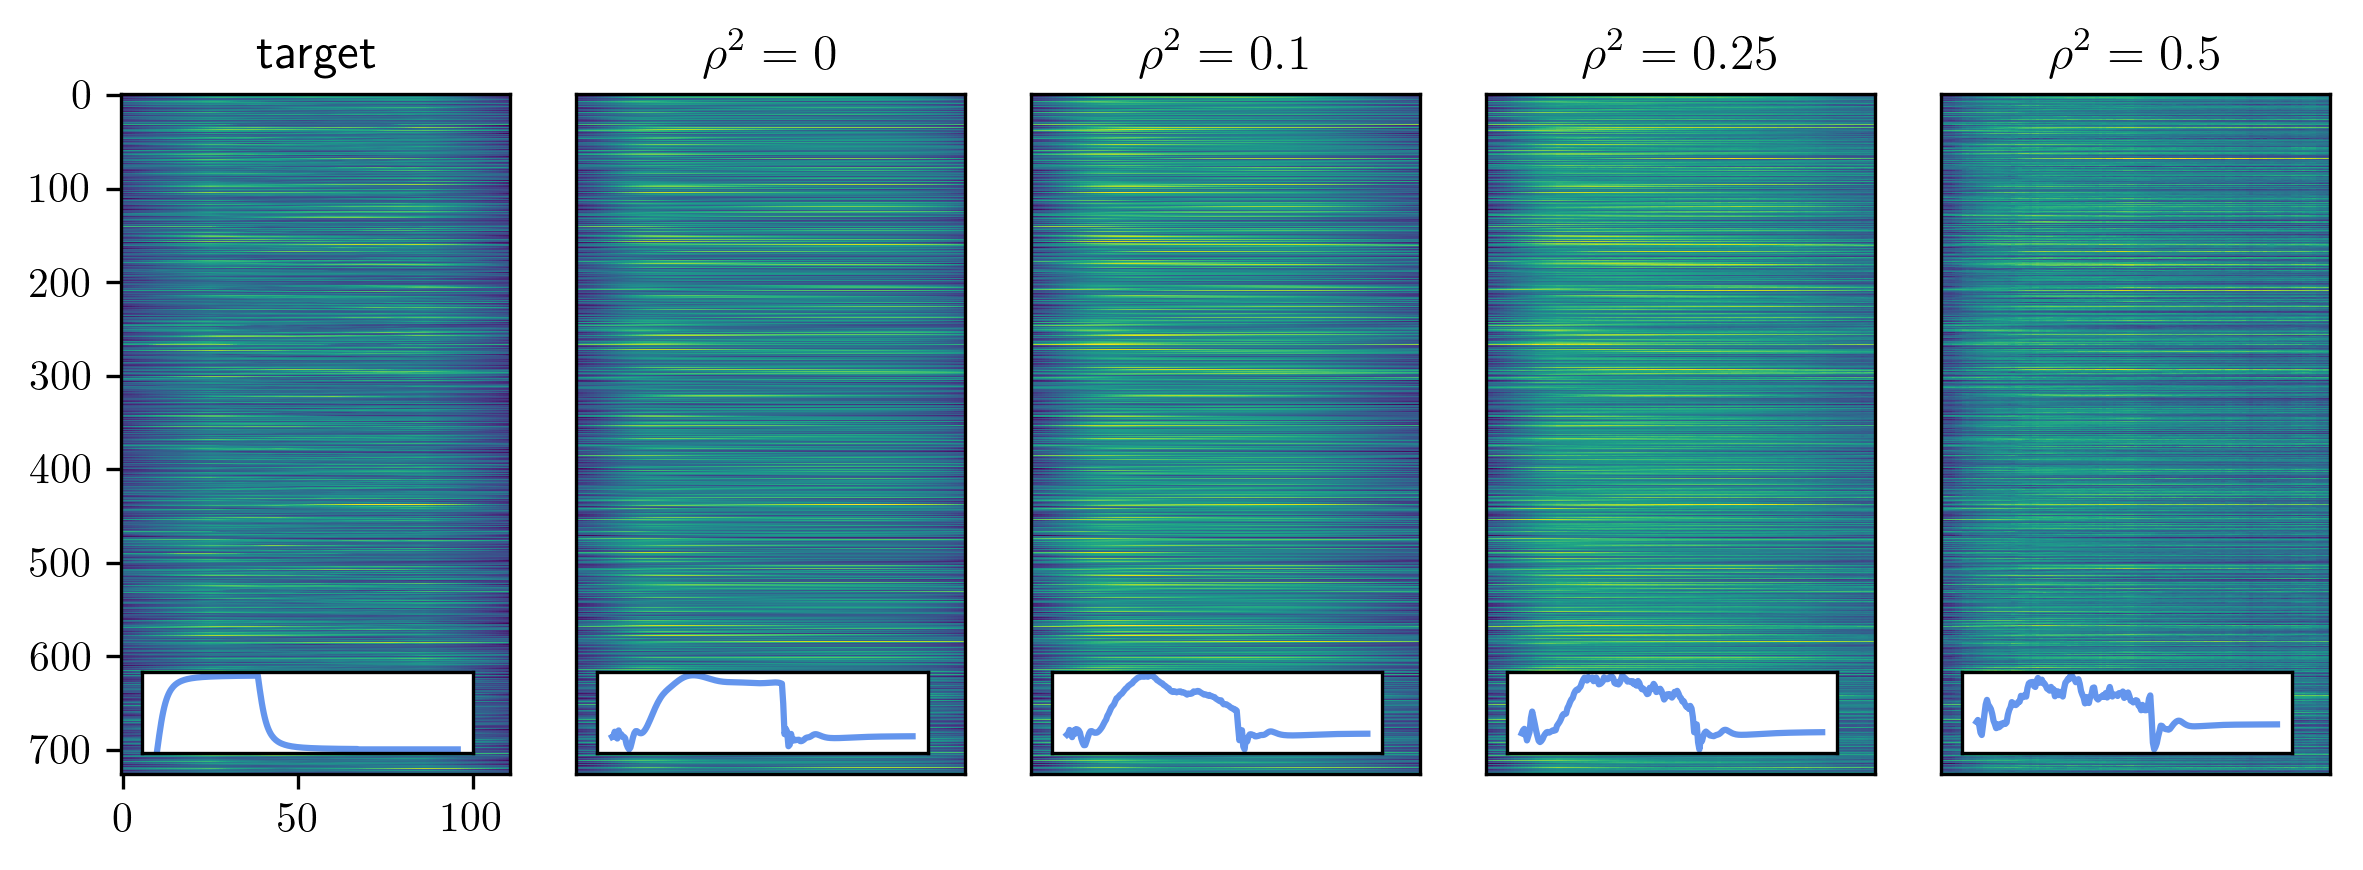
\includegraphics[width=\linewidth]{output_node_overlay.png}
    \caption{The output of a network trained with FORCE where the behavioral node is internal to the network. The target trace is compared to traces when the stimulus vector is corrupted by different levels of noise. The overlaid plots on each image represent the readout of the behavioral node.}
    \label{fig:my_label}
\end{figure}

We did this by introducing a target integrator node, whose activity was dependent on its own temporally anterior activations, and the anterior activations of other neurons in the network, but whose activity was not reintroduced into other neurons in the network at each time update (explained in more detail in \hyperref[sec:imp]{Implementation}). In other words, this target node integrated the firing patterns of other neurons in the network as well as its own firing patterns, but its output was not reintroduced into the network. In effect, the node's activity was dependent on other neurons in the network, but those other neurons were unaware of its presence in the network.
\begin{figure}
    \centering
    \includegraphics[width=\linewidth]{psychometric_curves.png}
    \caption{Network behavioral task variable response fit to psychometric curves acorss different amounts of noise corruption on the stimulus.}
    \label{fig:my_label}
\end{figure}

We found that network models were able to generate the correlated task behavior, even in the presence of strong stochastic noise on the sensory stimulus. In response to stimulus highly corrupted by noise, the networks' neural trace output began to decay significantly; interestingly, however, the target behavioral response remained accurate. Because the behavioral output node was designed to be an integrator of network activity, we performed a dimensionality-reduction analysis using principal component analysis (PCA) on model-produced neural data traces to attempt to understand how, even in response to highly noisy output the network is able to correctly determine the correct correlate behavior. 

\subsubsection{PCA analysis of target-producing network}
We found that trained network models were able to robustly generate target \emph{behavior}, in the presence of stochastically corrupted stimuli, even if networks' abilities to output \emph{neural data} were compromised.

Because the behavioral node of the network integrates the outputs of other nodes in the network, we expected to observe the trained model incorrectly reporting behavioral variables in response to noisy signals more frequently. This inspired us to investigate the underlying dynamics that give rise to the generation of neural firing patterns, both in the target neural traces, and in the outputs of the trained models, and how those dynamics influenced the generation of correlated task variables in the behavioral node. 
\begin{figure}[t]
 \centering
 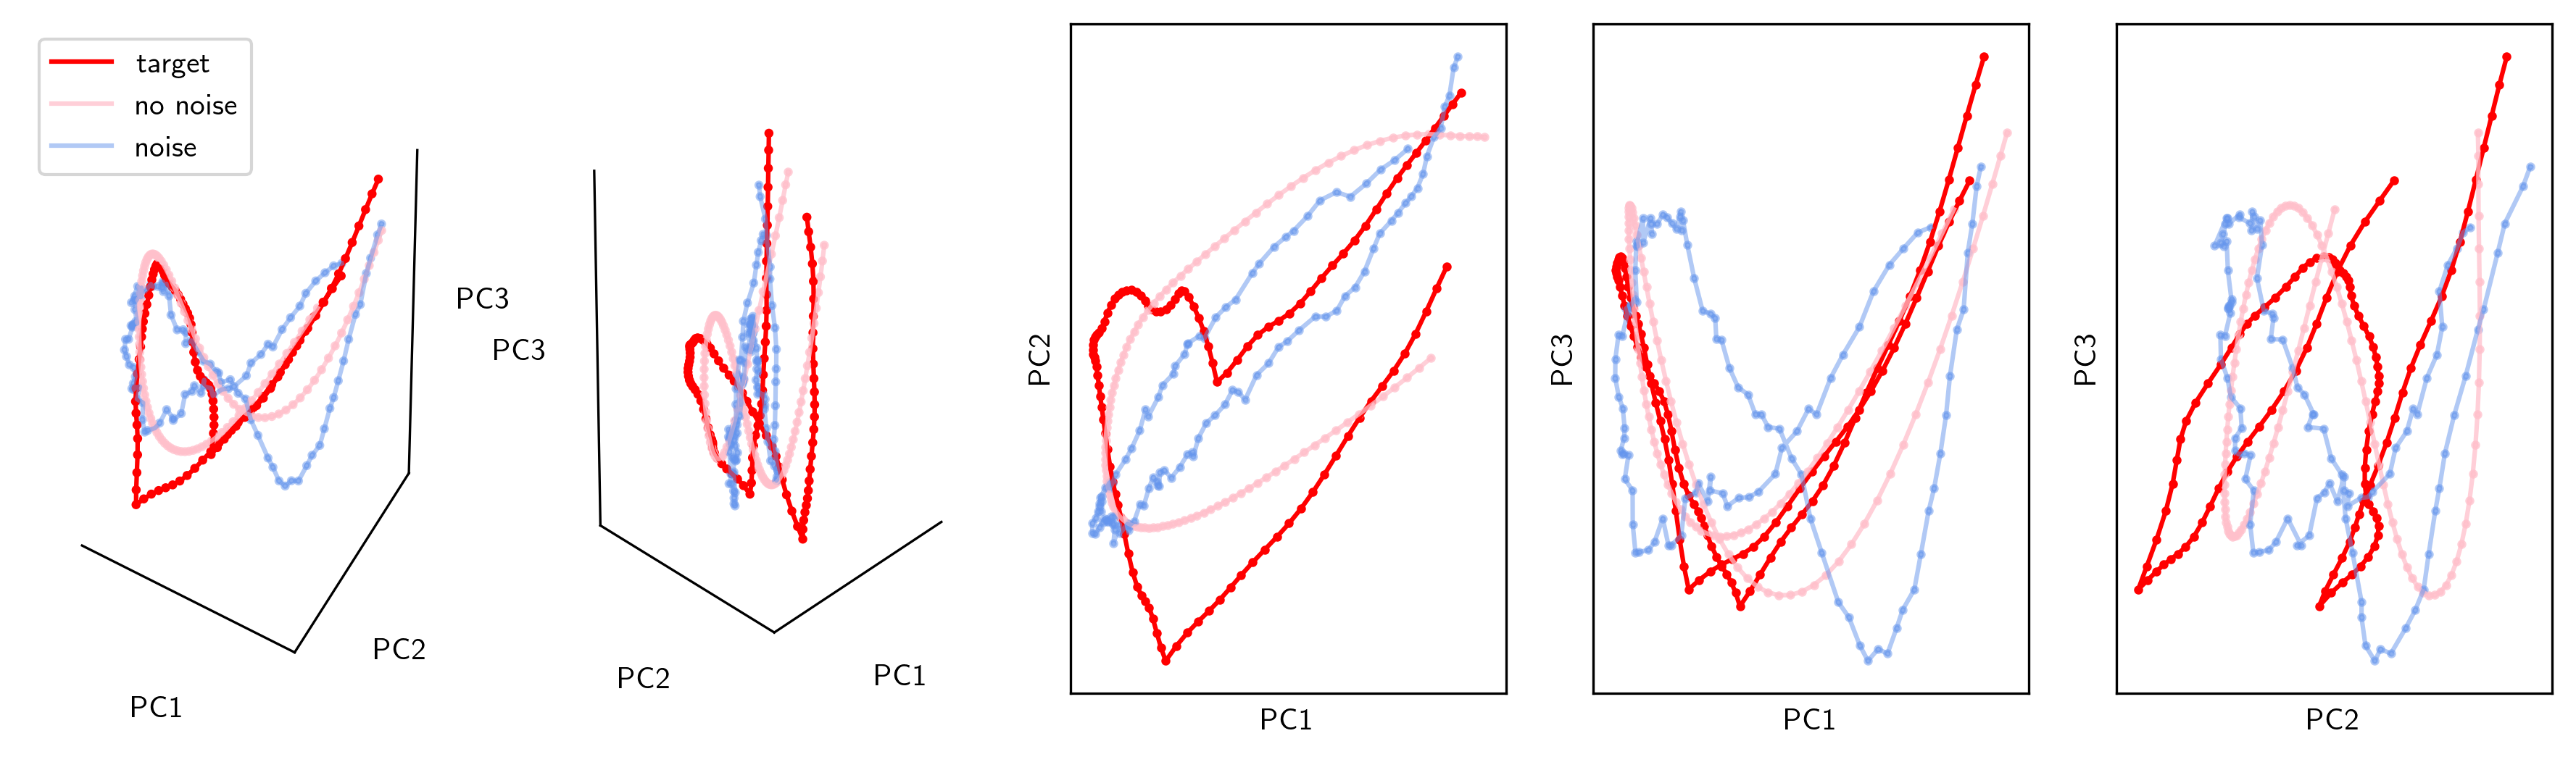
\includegraphics[width=\linewidth]{pca_noise_1.png}
 \caption{The PCA-projected network and target neuron activities over the course of an experiment of $T = 111$ ms. The left two traces show the progression of the neural activity projected onto the top $3$ principal components over time, and the right three traces show the progressions compared across $2$ principal components. These traces represent the projected neural data on trials where the monkey/network saw positive color coherence, negative motion coherence, and was instructed to report the color coherence.}
\end{figure}

We found that $\mathaccent92\%$ of the variance of both the neural data, and the neural traces output by trained network models, was captured in the top $3$ principal components of the aggregated firing rates across all time bins. We took advantage of this saturation of variance on the highest principal components to attempt to visualize the neural trajectories across the top $3$ principal components as a function of time, and analyzes these trajectories; namely, how they changed in the presence of stochastic noise accompanying the stimulus signal.

As demonstrated in \emph{Figure 8}, the collected neural data from the monkeys, and the output neural traces from the network evolve similarly over the course of stimulus presentation and integration, with the trajectories of dynamics across all three principal components remaining fairly idiosyncratic, even in the presence of noisy signals. More traces are presented in the Appendix B.

This suggests that the linear readout node that produces the target task variable may need only to track the oscillatory behavior between network output along $3$ (or slightly more) principal components in the system. The reduced dimensionality of this scheme provides an explanation for how, even in the presence of strong stochastic noise, the network is able to successfully discriminate neural data traces output by the network, even when they are obviously highly corrupted by noise.

\subsection{FORCE vs. full-FORCE}
Comparing FORCE and full-FORCE allowed us to gain insight into how differing training mechanisms, namely ones that are inspired with liquid/echo-state networks in minds, versus those that include the weight matrix of the RNN within the cost function, compare in terms of simulating neural data traces.

We found that the relative error using FORCE was smaller than full-FORCE in generating target neural traces. This was the case when the neural data traces were replicated on their own, and when the networks were trained to reproduce the target behavior both when decoding neural data fed into the network, as described in 6.2, and when the behavior generating node was a neuron within the network, as described in 6.3, as demonstrated in \emph{Figure 5} in the right panel.

\subsection{Localized linear dynamics}
After training the network models to generate the behavioral task variable \cite{CohenLol}, to reproduce the neural data recorded from the task, to generate the behavioral task variable in conjunction with producing the neural data traces, and inducing stochastic behavior in the network, we proceed to perform the localized linear dynamical analysis presented in \cite{BarakSussillo}, upon a model that more closely models the pertinent neural phenomena that we are investigating. 

\subsubsection{Identified slow and fixed points}
Optimizing $q({\bf x})$ (defined in \hyperref[sec:imp]{Implementation}) allowed us to located $41$ fixed points in the state space represented by the network's activities

When linearizing around fixed points in the system, we saw that the scheme demonstrated by \cite{Mante2013, BarakSussillo} breaks down. Notably, the eigendecomposition of the Jacobian of the network equation around fixed points failed to yield obviously orthonormal selection and integration vectors corresponding to an eigenvalue whose real part was $0$ or nearly $0$. Instead, across all fixed points and all trained networks, we routinely found that a large proportion of the real parts of the eigenvalues resulting from the eigendecomposition were $-1$, many were much less than zero, a few were fairly close to $0$, and some were positive, as demonstrated in \emph{Figure 9}, in the left panel.

This result prevented us from performing the same procedure outlined in \cite{BarakSussillo}, which, in their paper and in other papers that have used this method, has typically been performed on networks trained to due far simpler, lower-dimensional tasks than the one that our model was trained to do. In lieu of isolating the choice/selection axes that correspond to the the trained networks we used, we instead attempted to illustrate the mechanism through which the network is able to represent low-dimensional information in a high-dimensional state space, and shift behavior according to incoming stimuli. Because a great deal of variance in the activations was concentrated in the top $3$ principal components of the system ($\mathaccent89\%$), we chose to visualize the system as projected onto the top $3$ principal components in the the analysis that follows.

\begin{figure}
    \centering
    \begin{minipage}{0.49\linewidth}
        \centering
        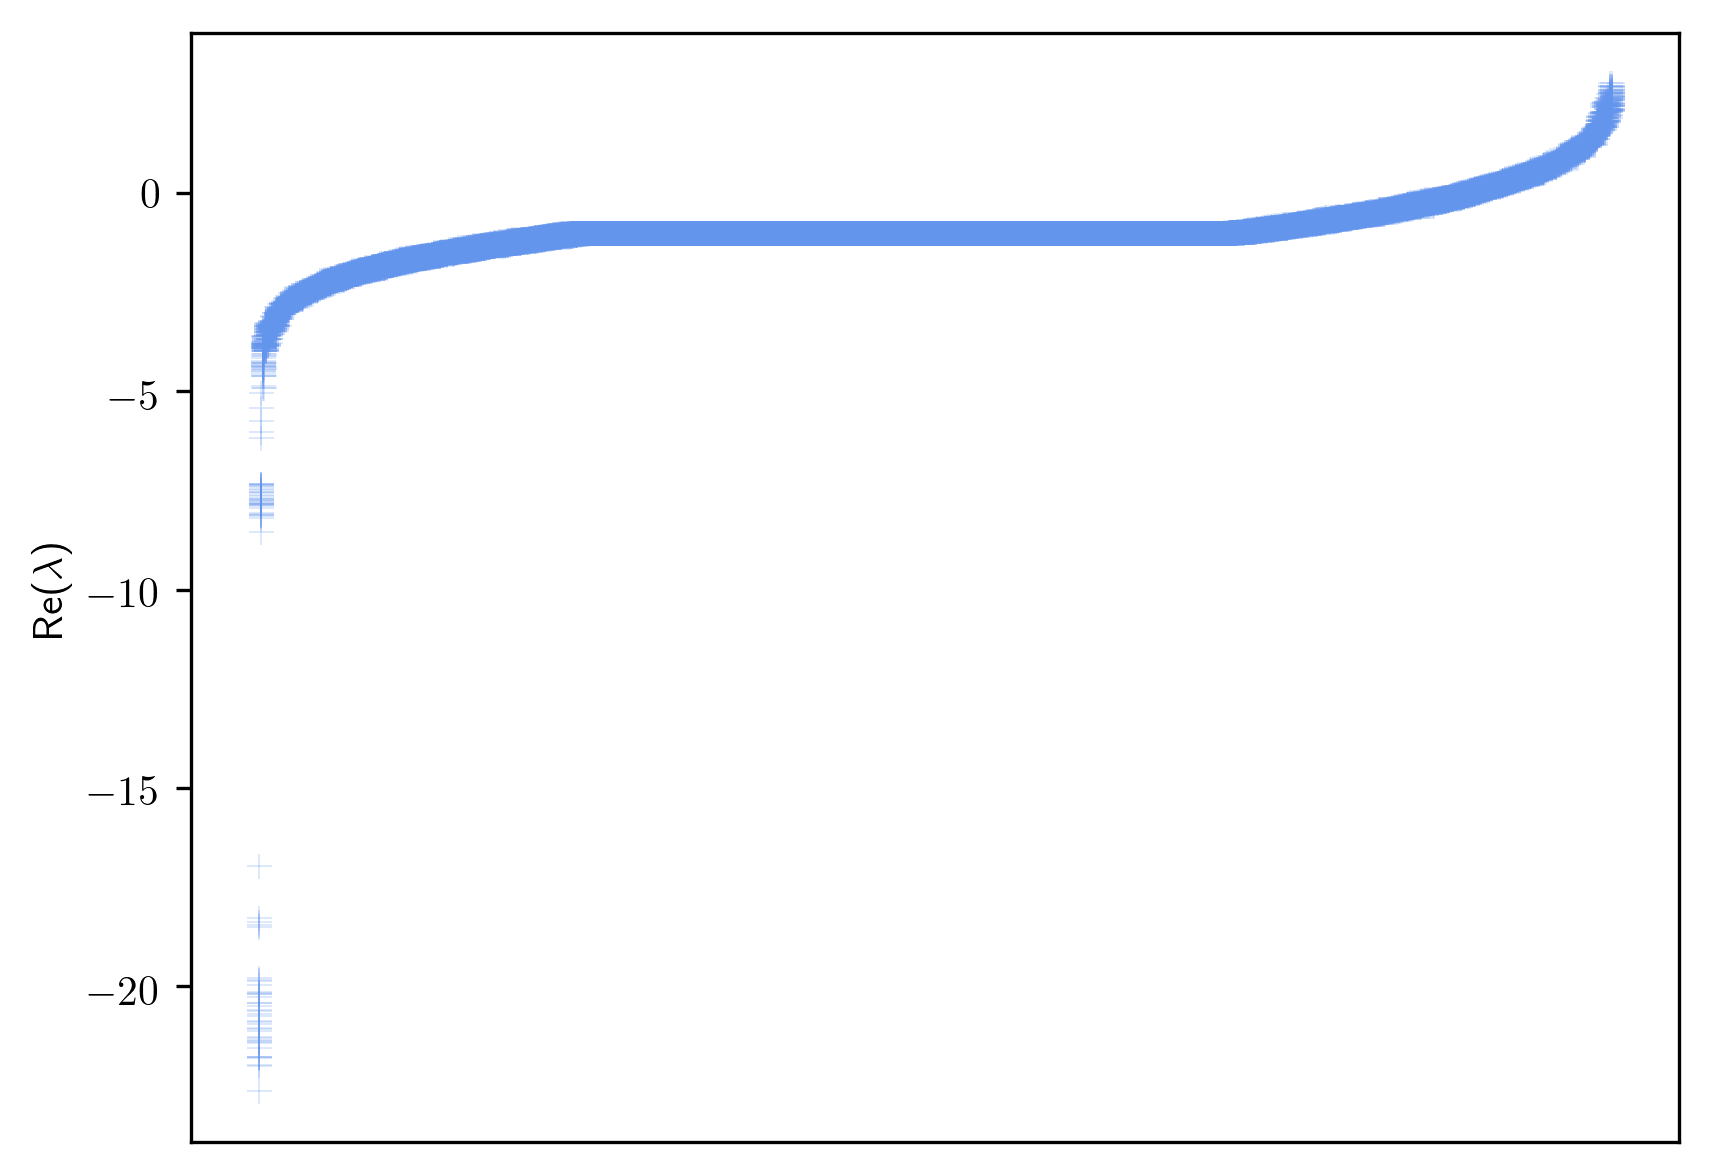
\includegraphics[width=\linewidth]{eigs.png}
    \end{minipage}
    \begin{minipage}{0.49\linewidth}
        \centering
        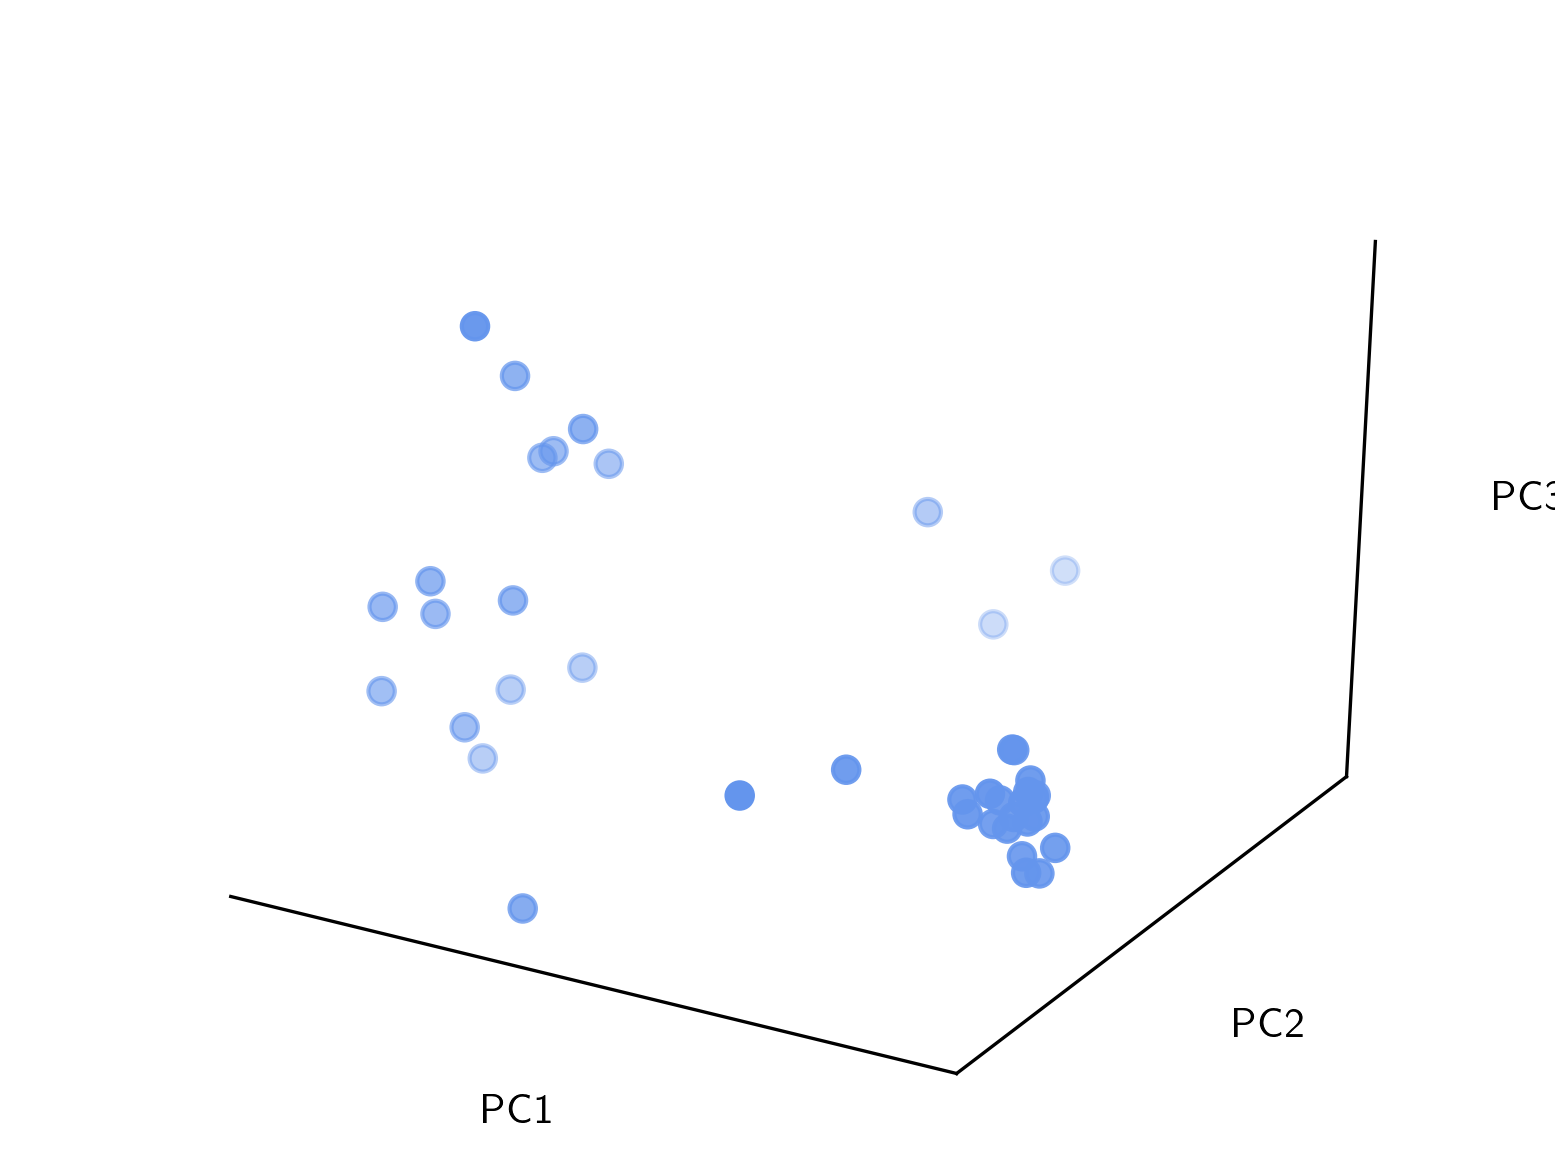
\includegraphics[width=\linewidth]{fixed_ps.png}
    \end{minipage}
    \caption{The right trace is a projection of the located fixed points onto the top $3$ principal axes. The left traces represents the distribution of real parts of eigenvalues found in the eigendecomposition of the network Jacobian around each fixed point.}
    \label{fig:my_label}
\end{figure}

\subsubsection{Phase space stitching via heteroclinic orbit tracing}
To demonstrate the versatility of the model, we attempted to drive the network between fixed points in the state space represented by the neural trajectories over several experiments, by driving the network to a fixed point, and presenting a stimulus coupled with a different fixed point in the state space. We traced the network trajectory as it travelled between these fixed points across the heteroclinic orbits connecting them.

\begin{figure}
    \centering
    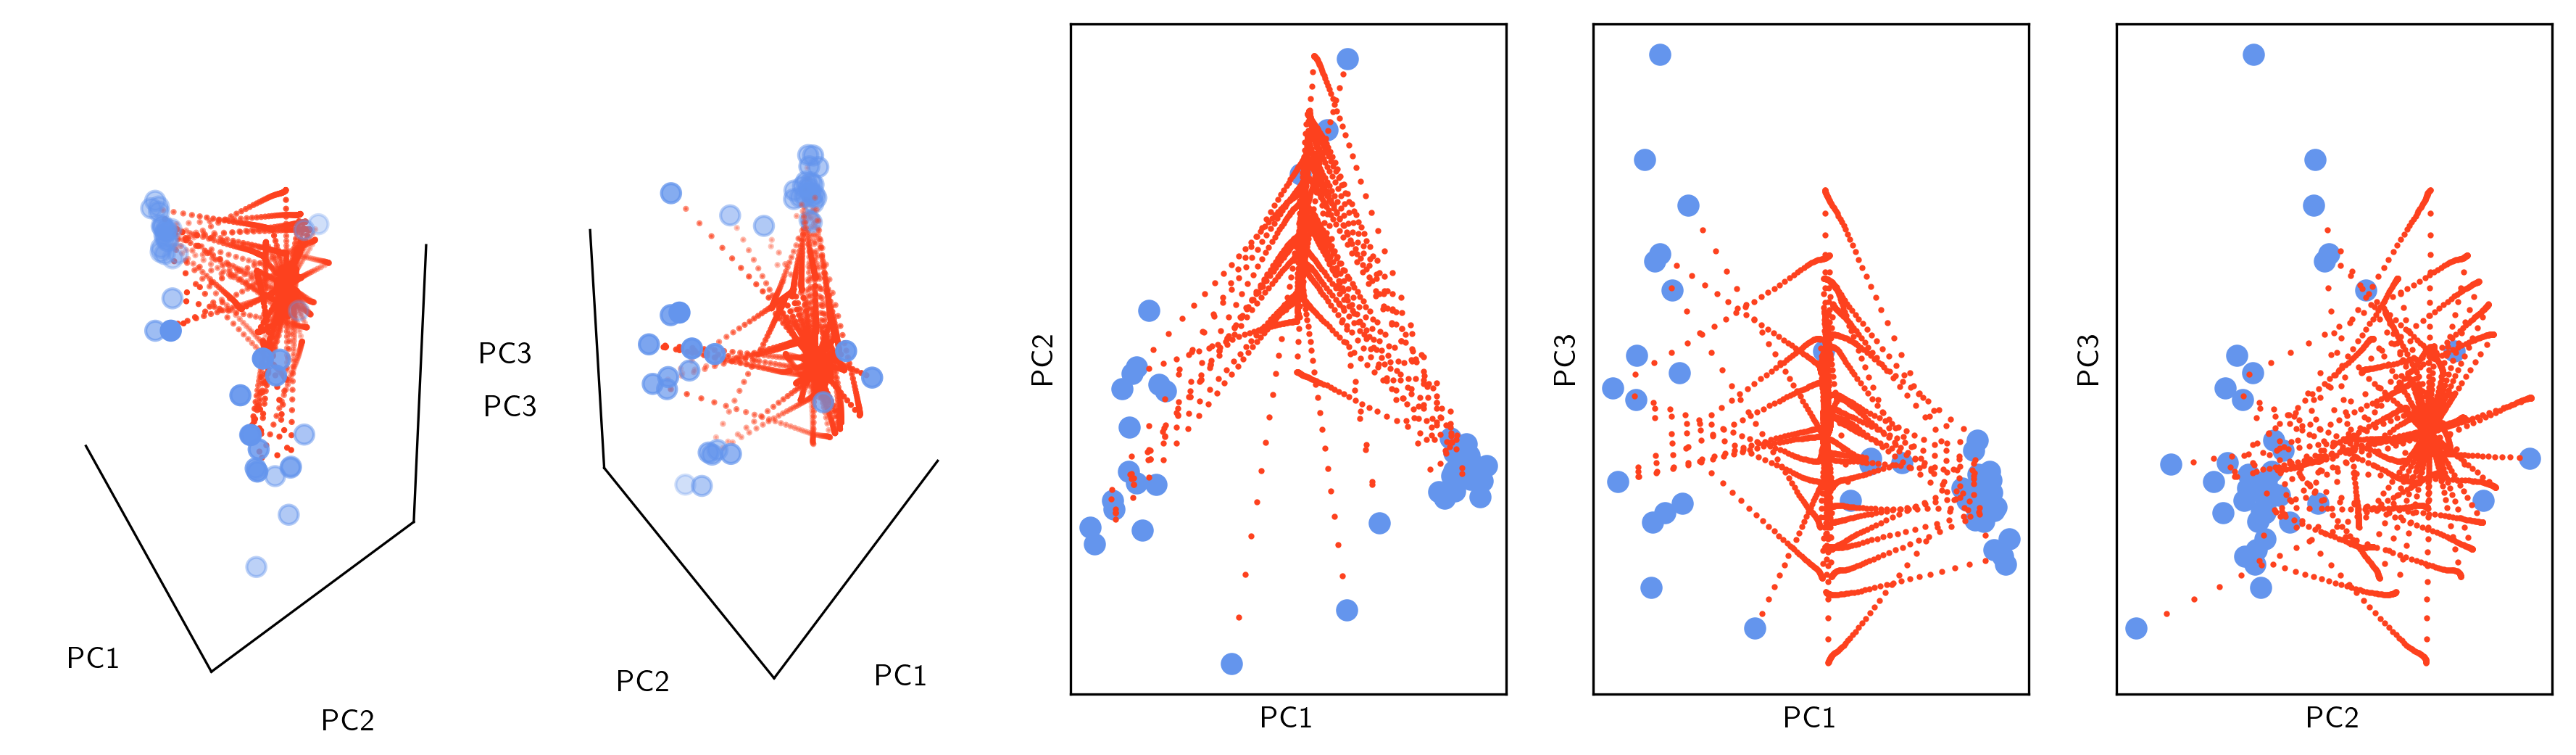
\includegraphics[width=\linewidth]{color_context_fixed.png}
    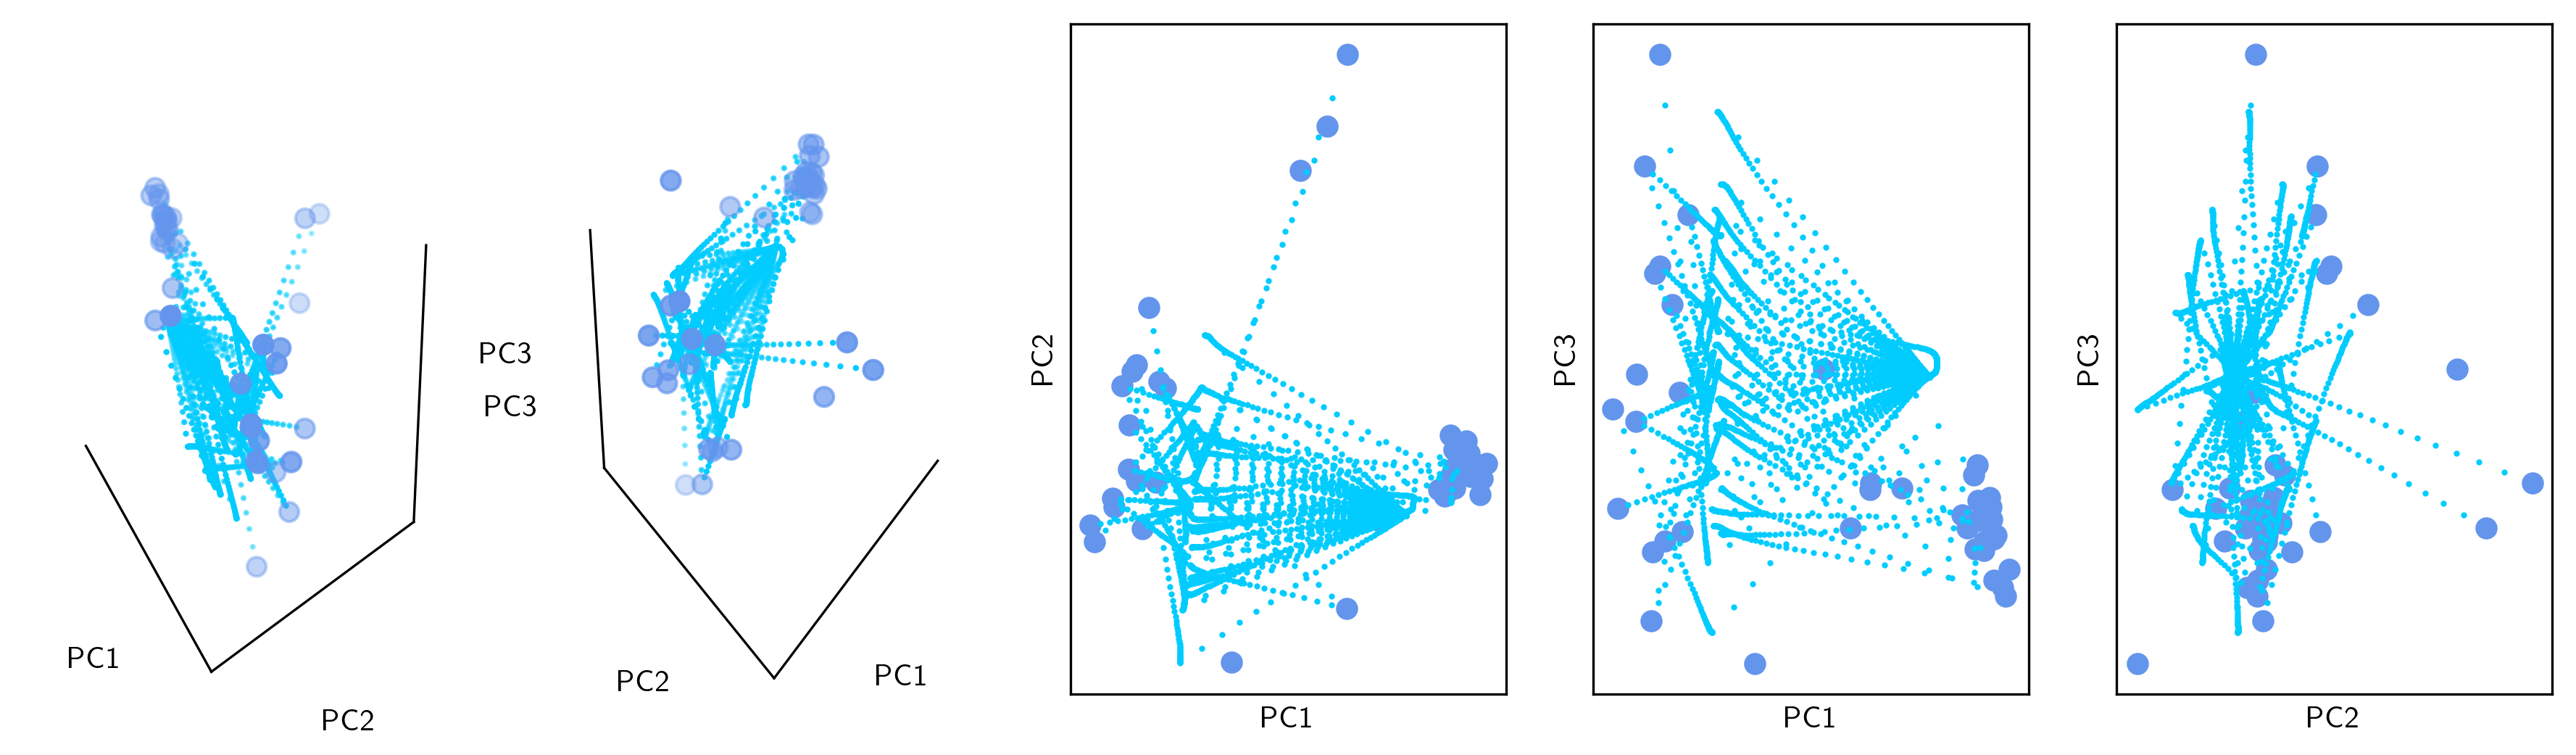
\includegraphics[width=\linewidth]{motion_context_fixed.png}
    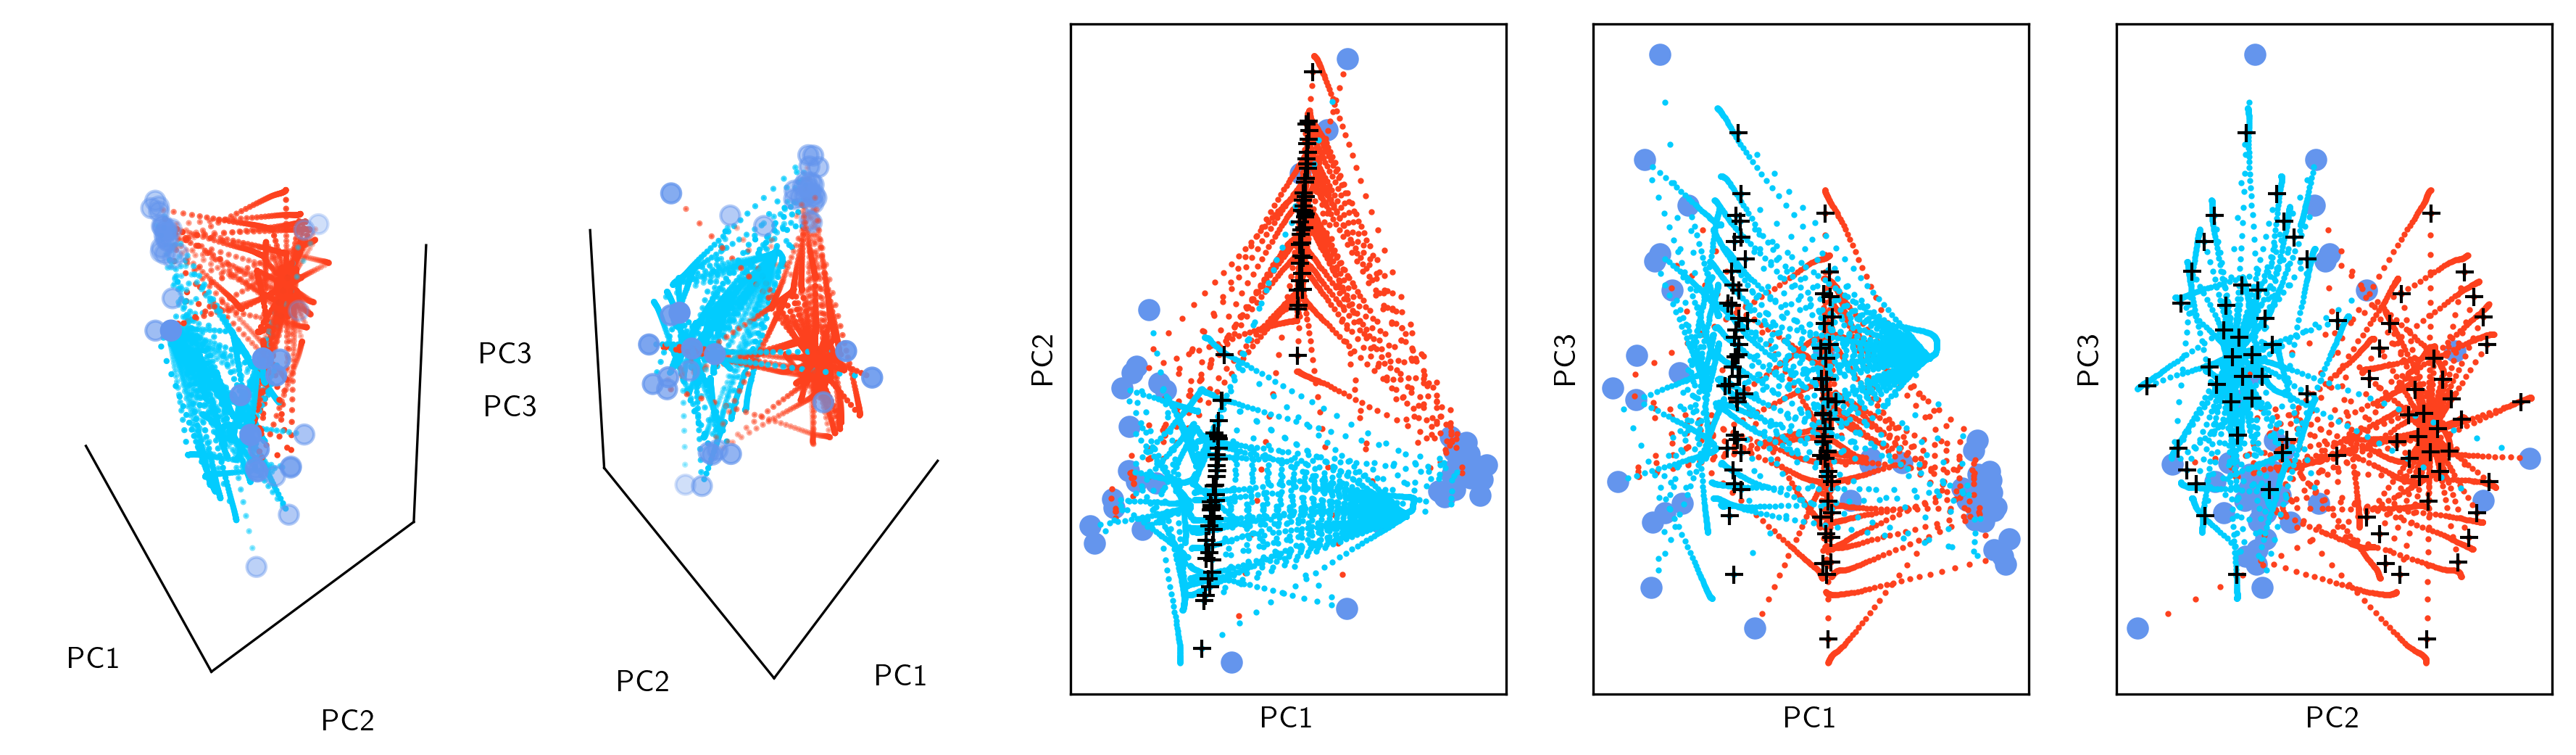
\includegraphics[width=\linewidth]{both_contexts.png}
    \caption{Traces of the network trajectories across fixed points that display heteroclinic orbits connecting them. The top trace is network trajectories over stimuli in the color context, the second row is network trajectories over stimuli in the motion context, and the final row is an overlay, with the approximate manifolds representing the stationary points for each context marked with black crosses.}
    \label{fig:my_label}
\end{figure}

We found that randomly initializing the network at a fixed point, and driving it with any combination of previously seen stimuli, often times drove the network into locally stable points in the system; often times, these wells either represented fixed points that the optimizer had not found (as the network theoretically has $72$ memory states, and, at the time of completing this report, we had found only $41$). In some cases, the network was perturbed into an energy well centered around a fixed point that we had explicitly uncovered. Once the network reached a neighboring fixed point, the trajectory represented by its activations projected into the reduced subspace spanned by the top $3$ principal components remained fairly stable, in some cases almost entirely stationary.

\begin{figure}
    \centering
    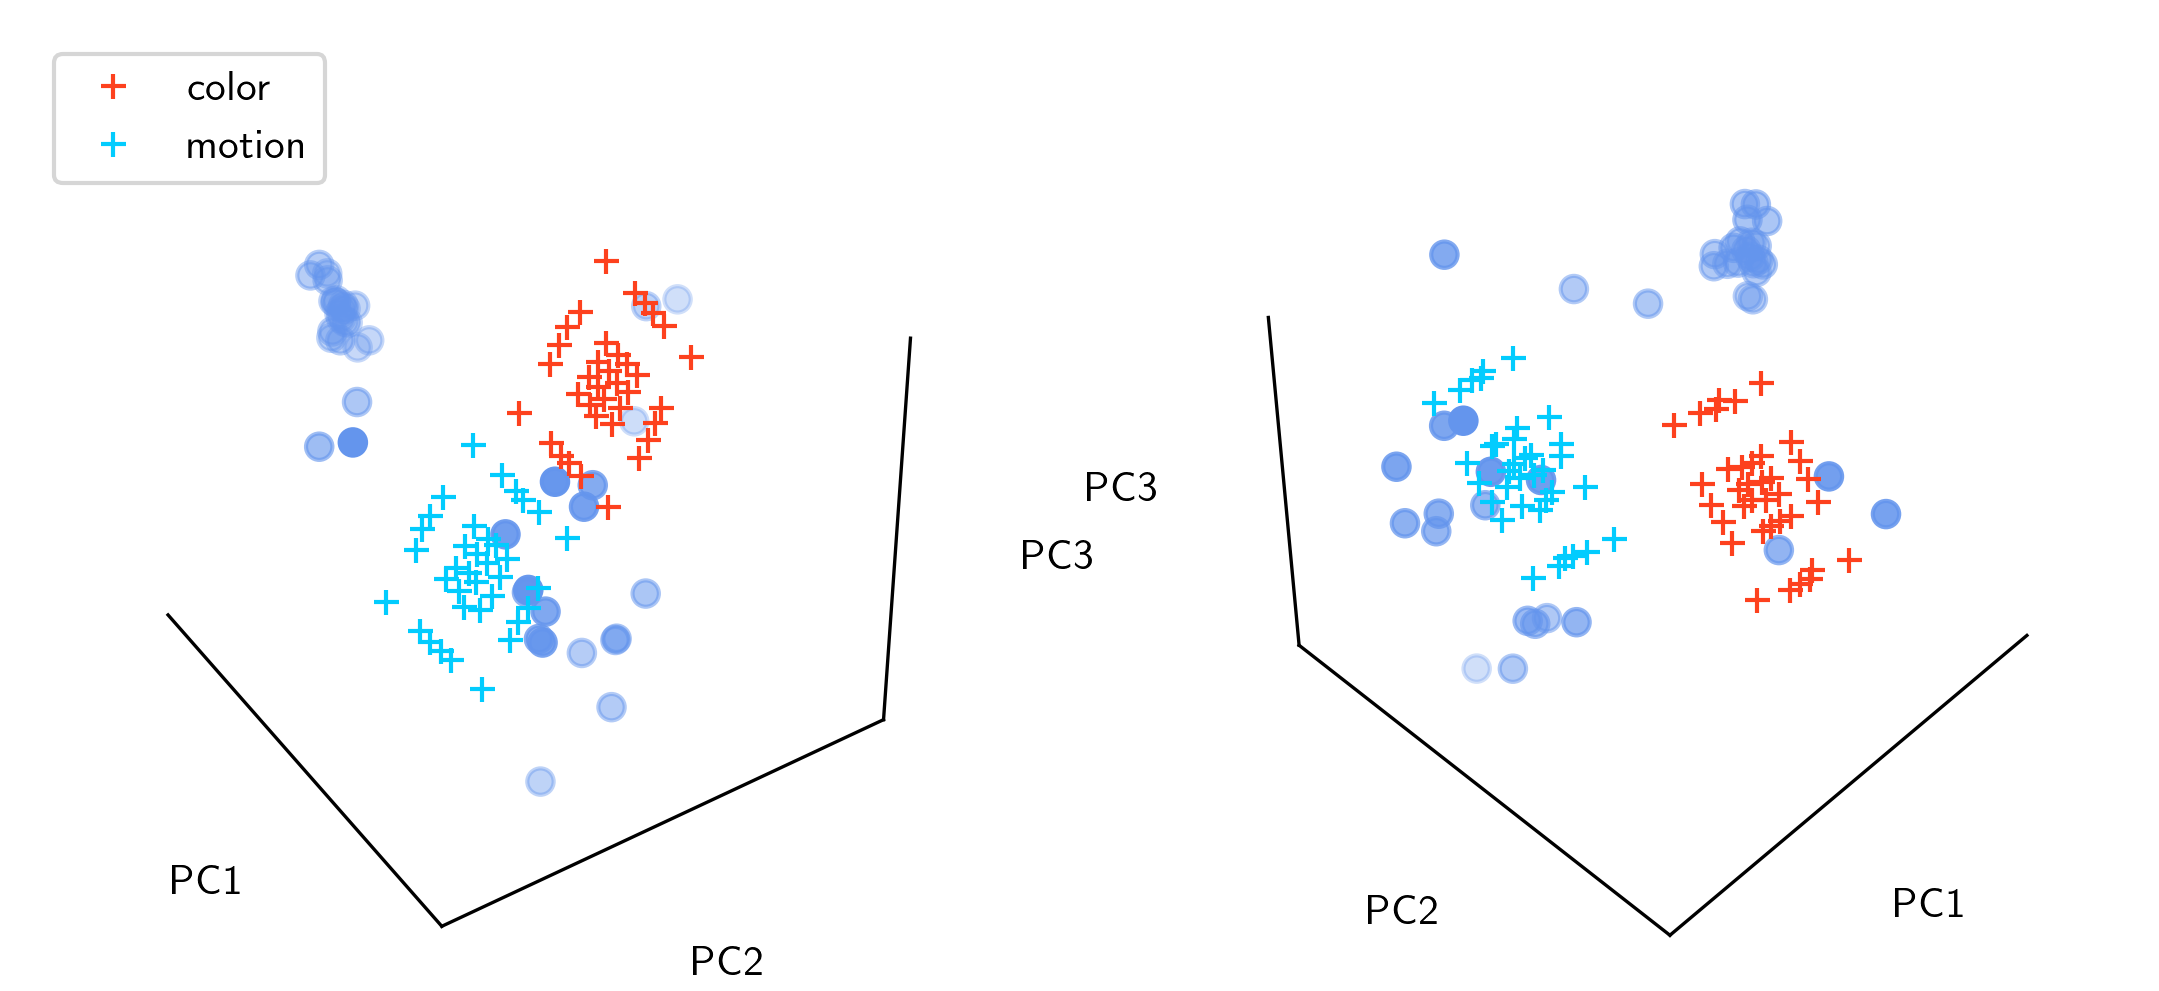
\includegraphics[width=\linewidth]{mid_trajectory.png}
    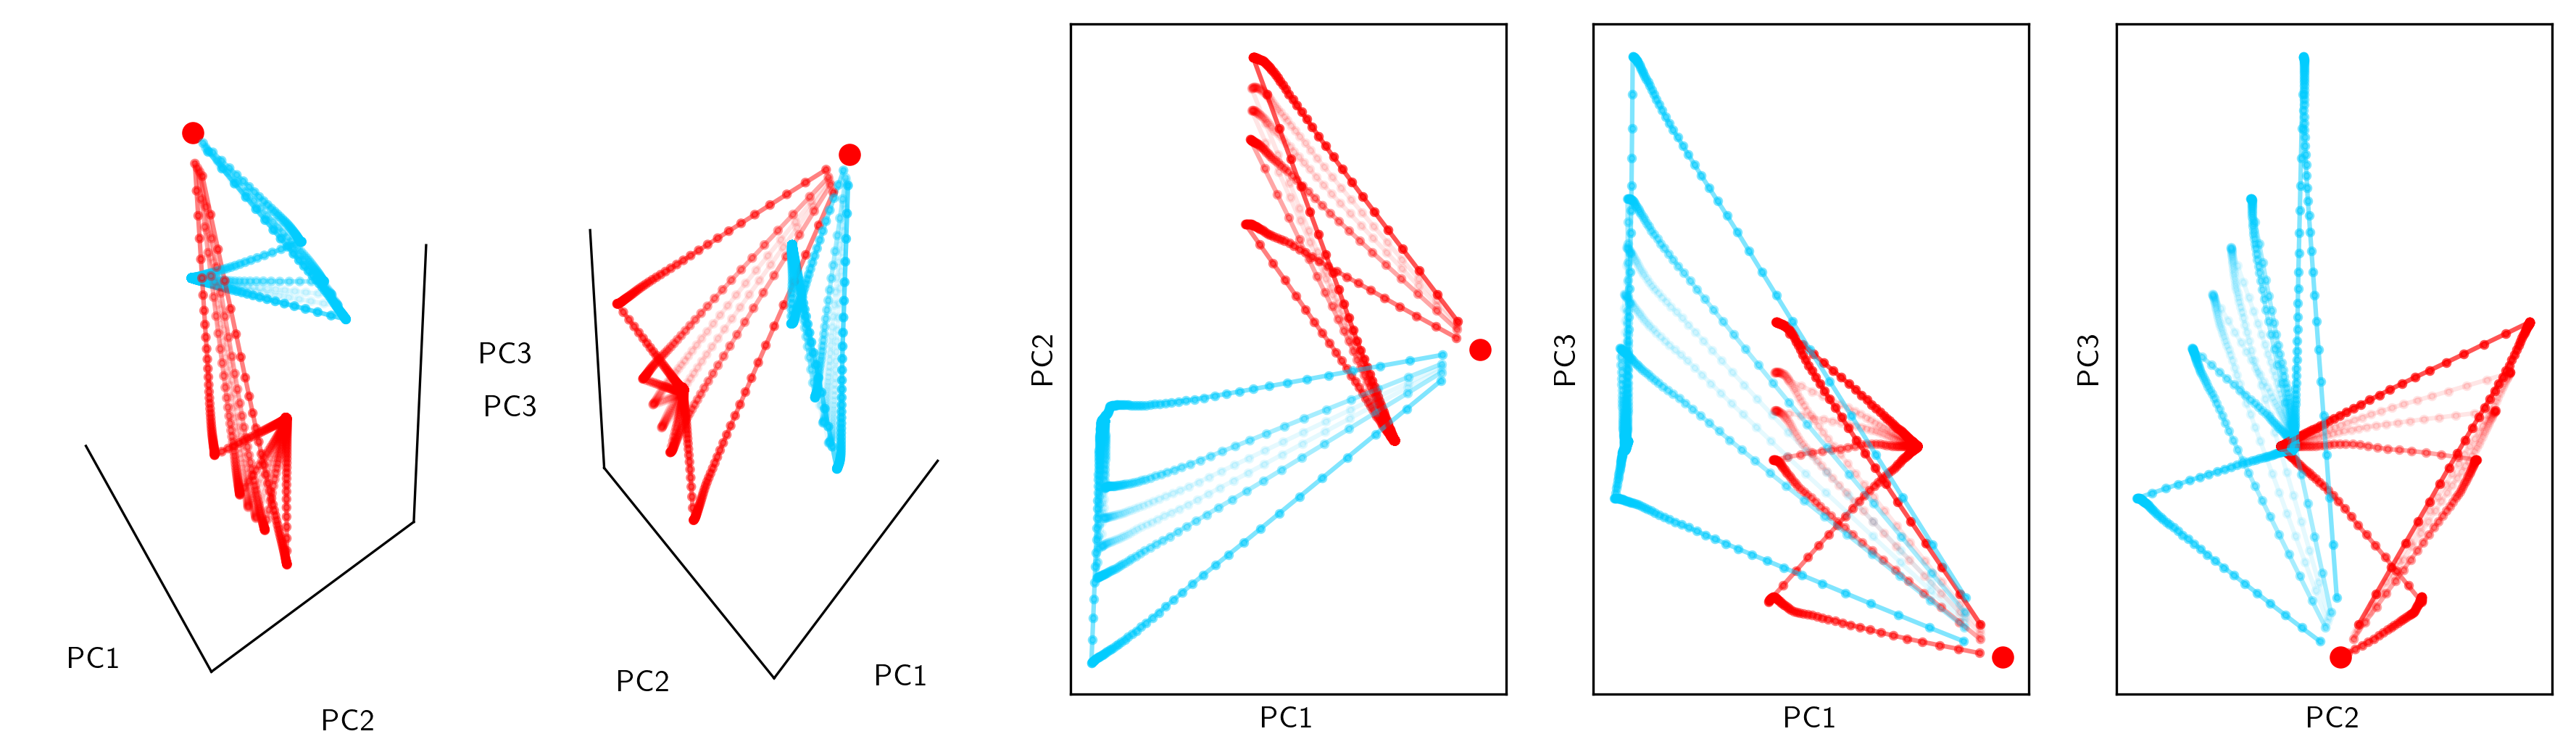
\includegraphics[width=\linewidth]{slow_points.png}
    \caption{The top traces display midpoints of the trajectories from \emph{Figure 10}, where the stimulus presentation ceased, demonstrating the approximate organization of stable points according to each permutation of stimuli, for both the color and motion contexts ($72$ in total). The bottom traces highlights the variance in network trajectories where the relevant stimulus value is held fixed (in either the motion or color context), and the irrelevant stimulus value is varied, demonstrating a slightly different trajectory for even differences in the irrelevant stimulus value.}
    \label{fig:my_label}
\end{figure}

This practice illustrates the way in which the network attempts to essentially ``learn'' a high-dimensional dynamical system flaked with several distinct wells, around which dynamics are approximately linear, and into which the network drives itself when presented with corresponding input stimuli. The readout of the network is dependent on the approximate location of the network in the state space, which, as demonstrated here, is entirely a function of input stimuli, the context cue, and the network's own recurrent non-linear activations.

As demonstrated in \emph{Figure 10}, stitching together the phase space of the trained network allowed us to gain deeper insight into roughly how the network was accomplishing the task of discriminating between relevant and irrelevant sensory inputs, and responding both in reproducing neural traces, and in producing the target behavioral task variable. In particular, this practice provided us with a visual indication of how the network organizes fixed points during training, and suggests an underlying mechanism for stimulus discrimination.

Note in the bottom row of \emph{Figure 10}; the projections of the network trajectories when initialized at a randomly chosen fixed point and perturbed with some arbitrary stimulus input for $50$ ms. The red traces are the network trajectories in the color context, and the light blue traces are the network trajectories in the motion context. A black mark indicates the position of the network activation in the state space at the moment the stimulus is turned off. 

Notably, the network, after training, appears to organize fixed and stationary points in the state space belonging the motion and color contexts in such a way that allows, on any axis in the subspace spanned by the principal components, for a hyper-plane to be drawn between them. In other words, identical stimuli (say, a strongly negatively coherent color stimulus and a strongly negatively coherent motion stimulus) drive the network into two fixed and linearly separable manifolds in the state space, along which the network progresses in time to generate the appropriate target task variable according to the dynamics local to the context-specific manifold in which it resides at the time when the target variable is reported. Dynamics along that manifold are idiosyncratic, and specific to the context that it represents.

To further understand local dynamics along this manifold, we isolated the points at which the network resides immediately after the stimulus is shut off, for all $72$ possible stimulus/context combinations, as shown in \emph{Figure 11}. The specific trajectories in the color and motion contexts are plotted beneath the $72$ points found in the state space for one specific set of six stimuli combinations (strong, negatively coherent color and varying coherence values of motion stimuli).

Unlike the scheme described in \cite{Mante2013}, irrelevant sensory data in a context still affects the ultimate trajectory of the network in the state space. In fact, irrelevant sensory data ultimately determines (along with relevant sensory data) where along the context-specific manifold the network is driven, as demonstrated in \emph{Figure 11}. The grid-like structure of the stable trajectories across both context-specfic manifolds roughly matches the relative strengths of the color/motion sense input data ($|0.5|$, $|0.17|$ and $|0.05|$).

This result, and its difference from that which is reported in \cite{Mante2013} ultimately makes sense: in the experiment in \cite{Mante2013}, the target function for relevant sensory data is held fixed according to varying strengths and coherence values of the irrelevant stimulus, and so it makes sense that the model network represents such information in a stereotyped way across all permutations of irrelevant sensory information. The task our network performed is not so simple; the neural traces the target was trained to produce were markedly different across conditions, even across different conditions in the same context and with the same value of relevant sensory input, and thus the network had to learn $72$ possible trajectories within the state space, rather than just $4$ ($2$, deflecting positive or negative, for either context).

\section{Discussion}
\label{sec:dis}
\subsection{Model capabilities}
Our network model is able to reproduce the target behavior we are studying, that of context-dependent feature discrimination, and do so with a level of accuracy that roughly mimics that of an animal subject. The network is also able to reproduce the neural traces gathered from macaque monkeys performing a context-dependent feature integration task, and thus, acts more as an explicit model for neural computation. Finally, the model is capable of integrating its own produced neural data traces, trained to match those of the macaque monkeys performing the task, and interpret these signals in such a way that allows it to ultimately generate the appropriate behavioral task variable. 

Thus, this paper makes an advance in the realm of modeling neural computation. Past models, like those in \cite{Mante2013} dealt entirely with reproducing the target behavior. Others, like in \cite{Rajan}, modeled neural population response, but in isolation of any correlated target behavior. Our model unifies these two approaches, arriving at a hybrid setup that more closely resembles how live organisms accomplish the many amazingly complex tasks that we routinely observe them to. The flexibility of these behaviors is largely a function of minute differentials in the coordinated neural firing patterns generated by neurons in the brain, and our model, building off of previous ones, exploits the richness of neural population responses in order to generate more complex, biologically relevant behavioral task variables.

Importantly, our model performs two steps of computational cognitive modeling: encoding information in the form of neural traces and decoding that information in the form of task behavior. In other words, our network model both simulates how information is represented in the brain via population responses, and also how that encoded information is then translated into correlated target behavior.

One advantage of bringing our model closer in likeness to the phenomena which it is actually modeling is that it allows us to make far less dubious claims about the nature of the systems we seek to analyze in greater depth. Namely, in crafting and testing a model of neural computation that can \emph{both} simulate neural firing patters and respond to those patterns and external stimuli, allows us to make inferential claims about how the brain accomplishes these context-dependent feature integration tasks (or, at the very least, begin to generate some intuition into how the brain is performing these tasks, while remaining reasonable). 

In what follows, we highlight in greater detail some results from this paper.

\subsection{Handling noise}
Important in understanding neural phenomena is simulating them beyond the deterministic realm. In other words, it is important for our model to sometimes incorrectly report the target task variable. In networks trained only to perform the task itself, it has been shown that it is possible to induce biologically realistic stochastic behavior \cite{CohenLol, Mante2013}. 

We show that in our model, which is designed to reproduce the target behavioral task variable \emph{and} the neural data recorded from monkeys performing the task, that stochastic behavior in the response variable is also possible to induce. In this paper, we set up the readout node responsible for producing the target behavior to be keyed into the neural traces that the network produces, which, in the presence of strong stochastic noise, begin to decay rather quickly. The network, however, is still able to reliably report the correct task variable. 

We performed PCA analysis on the network's output, which the integrator node directly integrates, in an attempt to understand the underlying mechanism for the read out node's ability to discriminate salient features even under high stochastic corruption. Our analysis demonstrated that most of the variance of the neural data traces is concentrated in the top three principal components. Traces generated by the network are stereotyped across these three components, even in the presence of a fair bit of stochastic noise. This result suggests that while the minutia of variances between neurons in the target traces certainly contribute to the target behavior, the output variable can be largely attributed to integration of neural traces and their fluctuations across $3$ axes in a reduced subspace of the neuronal activations.

These results demonstrate the possibility that, at least in the model, the learning task of integrating encoded information in the form of neural data and generating a target behavior can possibly be one of far reduced dimensionality than the structures of either the model or the brain inherently suggest. This ultimately makes sense, as while dynamics gain richness as dimensionality increases, the noisiness accumulated across higher dimensions can muddle a signal or encoded information beyond recognition. Perhaps within a reduced subspace, noisy signals, as represented in the brain, are learned over similar dynamics, thus making them not so much more difficult than noiseless ones to decode.

\subsection{The network as a high-dimensional dynamical system}
In this paper, we worked towards crafting a semi-quantitative view of how the model accomplished the task of integrating relevant and irrelevant sensory stimuli, and correctly discriminating between these stimuli to ultimately report the feature of interest. We characterized the model's ability to perform this task by treating the RNN as a high-dimensional dynamical system, one whose behavior is largely a function of its location in a state space tiled with several local linear regimes surrounding fixed points in the system. We demonstrated that the progression of the network, over time through the state space, is readily captured in a $3$-dimensional subspace, spanned only by the top $3$ principal components of the generated neural activity of the model. We also demonstrated that the flexibility of the network dynamics is due to the network's ability to flexibly travel between fixed points in its system, and oscillate within the energy wells surrounding to these points for as long as relevant sensory stimuli are being introduced into the network.

Our fixed-point analysis also lends us intuition for how the network model handles sensory information, both relevant and irrelevant. We demonstrated that the network's activities are context-dependent in the sense that identical stimulus information drives the network into one of two manifolds within the state space, one for each context (attend motion or attend color, in this case). We also showed that irrelevant sensory information \emph{does} have a bearing on the network's trajectory within the state space, determining where along the context-sensitive manifold the network arrives after integrating all sensory evidence. The target behavior that the network generates is not a result of ``filtering out'' irrelevant sensory information, so much as it is a result of the network's ability to represent releveat and irrelevant sensory information in a highly organized manner, and linearly (at least in a $3d$-subspace) separate context-dependent states.

Our results demonstrate that irrelevant sensory data does not decay away in the system, as described in \cite{BarakSussillo}, but rather remains within the system as it evolves. What determines the ultimate behavior of the network is not uniquely the relevant stimuli, but rather where the network drives itself, depending on context, in the state space. The location of the network is necessarily dependent on the irrelevant stimulus just as much as the relevant stimulus. The task of representing sensory information within the system, then, is not discrimination via deletion of irrelevant stimuli, but rather incorporation of relevant and irrelevant stimuli, and stereotyped behavior depending on the location of the network on a manifold corresponding to the context that the network is in.

\section{Conclusions, limitations and future work}
\label{sec:con}
In this paper, we present a model for neural computation, one that is capable of learning and generating target behavioral variables aligned with a context-dependent feature discrimination task, the neural traces measured from monkeys performing the task, and integrating these neural traces into a target behavioral readout. 

By crafting a model that is able to closely mimic model neural behavior, we bring ourselves one step closer to making inferential claims about feature integration in neocortex, or at least in understanding rudimentary underlying mechanics for complex neural functions. We found that our network model was able to represent context-dependent sensory information by way of organizing fixed trajectories in a high dimensional state space along manifolds corresponding to relevant sensory contexts. We demonstrated that our model did not filter our irrelevant sensory data, but rather incorporated it into its eventual trajectory along the dynamical system. This suggests an underlying mechanism for feature integration that is similar to that presented in \cite{Mante2013}, but also different. 

Importantly, our model demonstrates that the linearized analysis around fixed points fails when the output function is high dimensional and complex, like neural data. This suggest that feature integration in the brain follows a murkier path than that presented in \cite{Mante2013}; while the simplification to orthogonal choice and selection axes provides intuition that is helpful in understanding feature integration in general, it must and can be enhanced when complicating and enriching the target behavior of the network model, as has been done in this study.

\subsection{Limitations}
Our work is primarily focused on building a model for neural computation. We are hindered, in that respect, by the set-up of our model, which trains a network to reproduce several target functions with respect to weights that are external to the actual network itself. The brain has no such setup: all behavior and neural activations are mediated solely by the firing rates and synaptic connections between neurons. This opens a larger, philosophical question in the area of research, which often trains models that achieve target behavior via learning weights external to the network, but also compels us to consider training techniques and model constructions that even more closely mimic neural functioning as we understand and observe it. 

Additionally, the training procedure we employed was a supervised method. While this allowed us to achieve high accuracy in our model, it is ultimately an unrealistic training procedure for mimicking neocortical learning: there is no ``target function'' that the brain seeks to learn, and no error feedback into the brain that allows it to approximate that function. In search of computational expediency and in order to reliably generate an exact match of the target behavior we are studying, we resorted to a supervised learning method. However, this limits our ability to make correlate claims about brain function, as it places far too heavy of an assumption on how the brain learns. 

\subsection{Future work}
In future work, we can address some of the limitations proposed in this section in order to bring ourselves closer to a model for neural computation. The recent development of unsupervised learning mechanisms and generative models via deep learning methods \cite{SussilloLFADS} unlocks a whole new sector of cognitive modeling. Instead of teaching a network how to precisely mimic a target behavior, future work can focus on teaching a network a latent distribution over potential neural activities in response to incoming sensory information, and then investigate the underlying structure of the latent distribution, as well as the generative examples that the model generates.

Additionally, we can train more complex, multi-layered models that more closely mimic how we have observed the brain to function. Recent advances in pairing spiking networks and networks like those used in this paper, which model population averaged responses, have demonstrated a remarkable capacity for learning complex behaviors, like sequence generation and temporally dependent tasks \cite{SussilloLFADS}. These compiled models also allow for finer tuning of the model; for example, in the foreseeable future, models that don't rely on the learning of weights external to the network will grow in popularity in cognitive modeling, and we can use them to make more precise claims about how the brain integrates and represents information. In general, inferential claims made about the brain via modeling are highly contingent upon the biological relevance of the models used. The closer we can bring models to their neural correlates, the stronger our claims about cognitive functioning can be.

Ultimately, this work represents a small step in understanding various aspects of neural computation, particularly with regard to how context-dependent information in the brain is computed and represented with regard to a specific goal state, and paves the way for future research into the subject.

\newpage

\section*{Acknowledgments}
I would like to thank my adviser, Prof. Jonathan Pillow, for introducing me to the topic of dynamic neural computation, and for encouraging me to pursue this project. The learning curve for this material was steep, but the invaluable advice and guidance I received along the way made the work in this paper possible. 

I would also like to thank Brian DePasquale for his help in pivoting us towards investigating the full-FORCE procedure, and for providing deep insight into the nature of the techniques surveyed in this paper.

\medskip

\section*{Pledge}
This paper represents my own work in accordance with University regulations.

/s/ Zach Cohen

\printbibliography

% {\setstretch{1.0}
% \small
% \listoffigures
% }

\newpage

\section*{Appendix A: Recursive least-squares (RLS) filter}
The purpose of the RLS filter is to generate some filter weights ${\bf w} \in \mathbb{R}^{m \times n}$ that map some inputs ${\bf u} \in \mathbb{R}^{m \times n}$ to some desired responses ${\bf d} \in \mathbb{R}^{m \times n}$ to minimize the sum of squared errors over each weight $i = 0\dots n$:
\[
    \mathcal{E}(n) = \mathcal{E}((w_0(n), \dots w_{m-1}(n)) = \sum_{i = 1}^n \beta(n, 1)[d(i) - \sum_{k = 0}^{m - 1}w_k(n)u(i-k)]^2
\]
and where the error signal is $e(i) = d(i) - y(i) = d(i) = \sum_{k=0}^{m-1} w_k(n)u(i-k)$. For this paper, we use an RLS rule that employs some forgetting factor, $\beta(n,i) = \lambda^{n-1}$. The forgetting factor can be thought of how ``strong" the memory of the filter is, or else, how far into the future (if we consider time-dependent data) some observation at time $t$ and influence the weights when determined at some time $t + \epsilon$. 

We can determine the solution that minimizes $\mathcal{E}(n)$ by using the least-squares solution. Renaming variables such that: $u'(i) = \sqrt{\lambda^{n-i}}u(i)$, $d'(i) = \sqrt{\lambda^{n-i}}d(i)$ and $\beta(n,i) = \lambda^{n-i}$:
\begin{align*}
    \mathcal{E}(n) &= \mathcal{E}((w_0(n), \dots w_{m-1}(n)) = \sum_{i = 1}^n \beta(n, i)[d(i) - \sum_{k = 0}^{m - 1}w_k(n)u(i-k)]^2 \\
    \mathcal{E}(n) &= \sum_{i = 1}^n [d'(i) - \sum_{k=0}^{m-1}w_k(n)u'(i-k)]^2 \\
    \boldsymbol{\mathcal{E}} &= \lVert \boldsymbol{D} - \boldsymbol{W} \boldsymbol{U} \rVert ^2
\end{align*}
which is the standard least-squares criterion. Then, $w(\cdot)$ can be written as:
\begin{align*}
    {\bf w} &= ({\bf u}^T {\bf u})^{-1} {\bf u} {\bf d} \\
    &=\big((\sum_{i=1}^n\lambda^{n-i}u(i)^Tu(i))^{-1}\big)\sum_{i=1}^n\lambda^{n-i}u(i)d(i) 
\end{align*}
and for brevity, we denote $\sum_{i=1}^n\lambda^{n-i}u(i)^Tu(i) = \Psi(n)$ and $\sum_{i=1}^n\lambda^{n-i}u(i)d(i) = \phi(n)$.

To recursively determine the solution (over, say, some time period), we compute $w(n) = \Psi(n)^{-1}\phi(n) \Leftrightarrow w(n-1) = \Psi(n-1)^{-1}\phi(n-1)$, and thus:
\begin{align*}
    \Psi(n) &= \lambda \Psi(n-1) + u(n)u(n)^T \\
    \phi(n) &= \lambda \phi(n-1) + u(n)d(n)
\end{align*}
Thus, we have our update equations for two important quantities, except that we want $\Psi(n)^{-1}$, rather than $\Psi(n)$. To obtain it, we use the matrix inversion lemma: if $A = B^{-1} + CD^{-1}C^T$, then $A^{-1} = B - BC(D + C^TBC)^{-1}C^TB$, and so
\[
    \Psi(n)^{-1} = \lambda^{-1}\Psi(n-1)^{-1} - \frac{\lambda^{-2}\Psi(n-1)^{-1}u(n)u(n)^T\Psi(n-1)^{-1}}{1+\lambda^{-1} u(n)^T\Psi(n-1)^{-1}u(n)}
\]
which is our update equation for $\boldsymbol{P}(t) \equiv \Psi(n)^{-1}$. The other terms are defined by letter $e(t) = d(n) - u(n)^Tw(n-1)$, mixing notation from this explanation and the introduction of FORCE and full-FORCE in the paper \cite{Hayes}.

\newpage

\section*{Appendix B: Remaining PCA trajectories}
The following are the remaining PCA trajectories recorded (see section 6.3.1 for details).
\begin{figure}[h!]
    \centering
    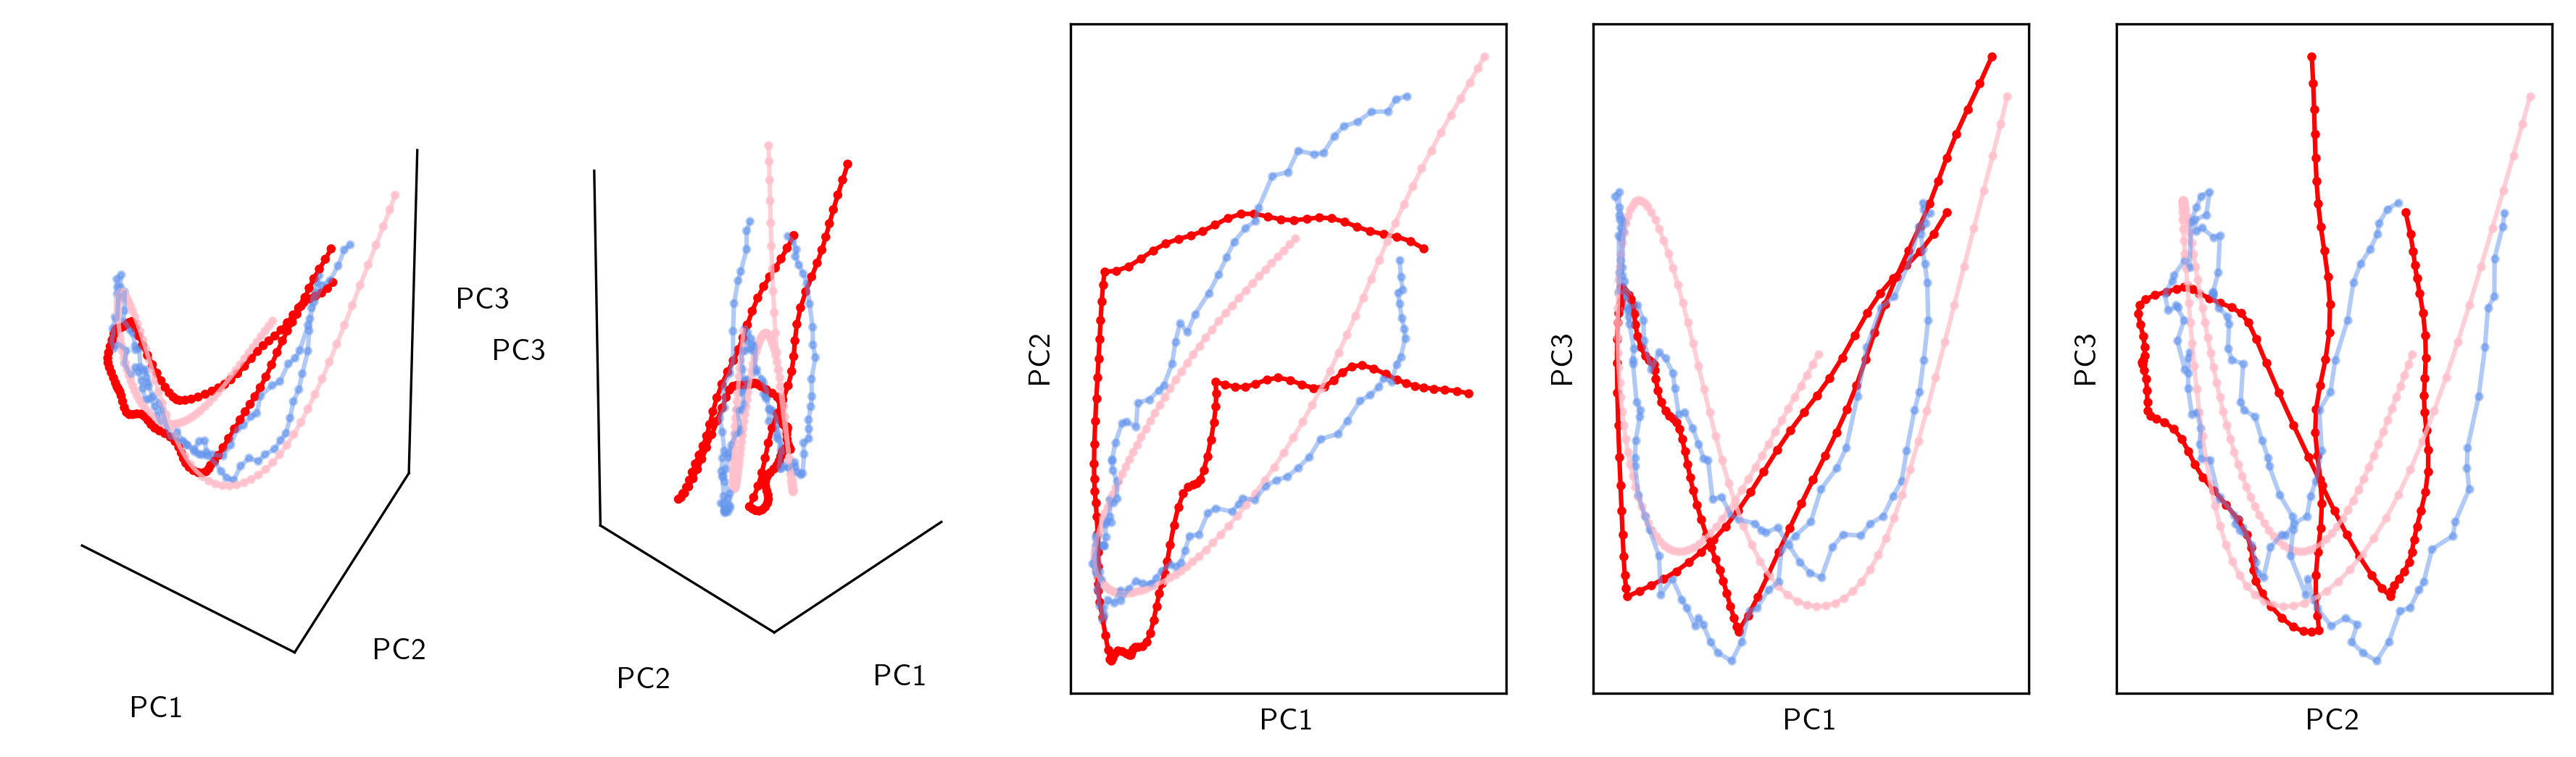
\includegraphics[width=\linewidth]{pca_noise_2.png}
    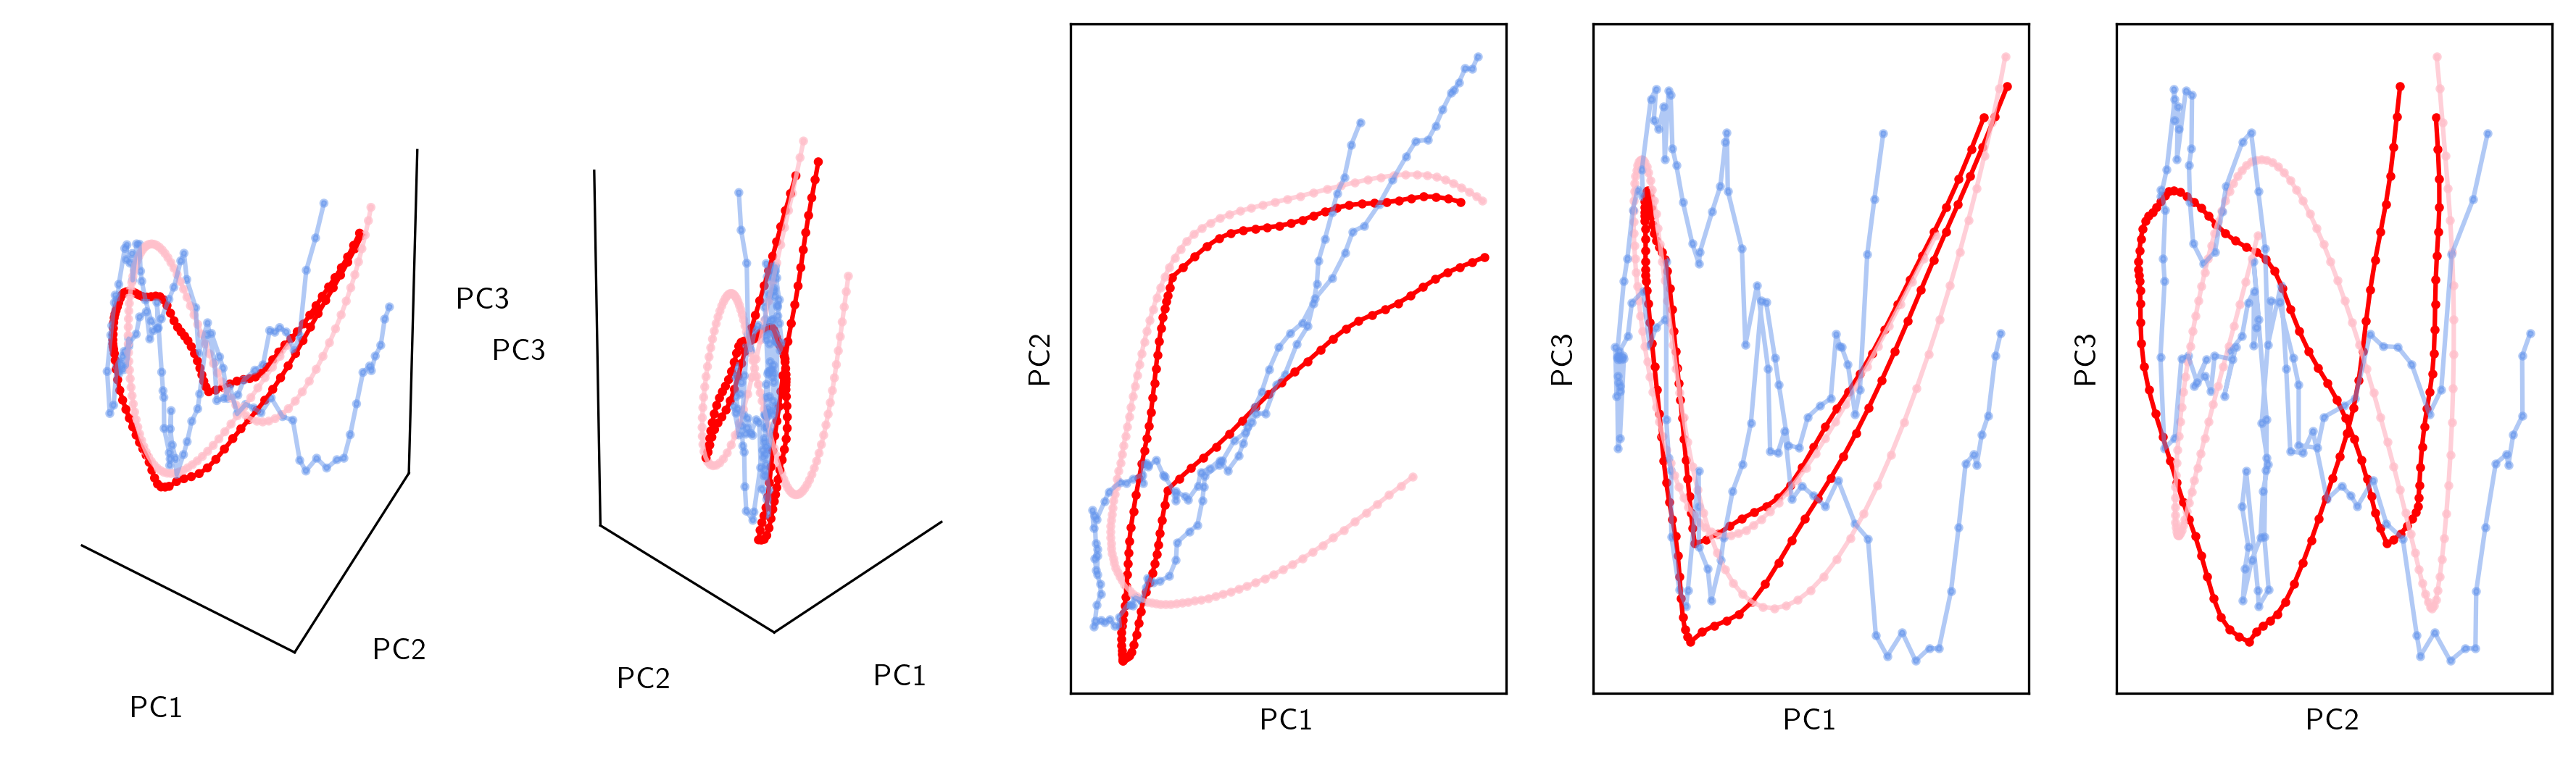
\includegraphics[width=\linewidth]{pca_noise_3.png}
    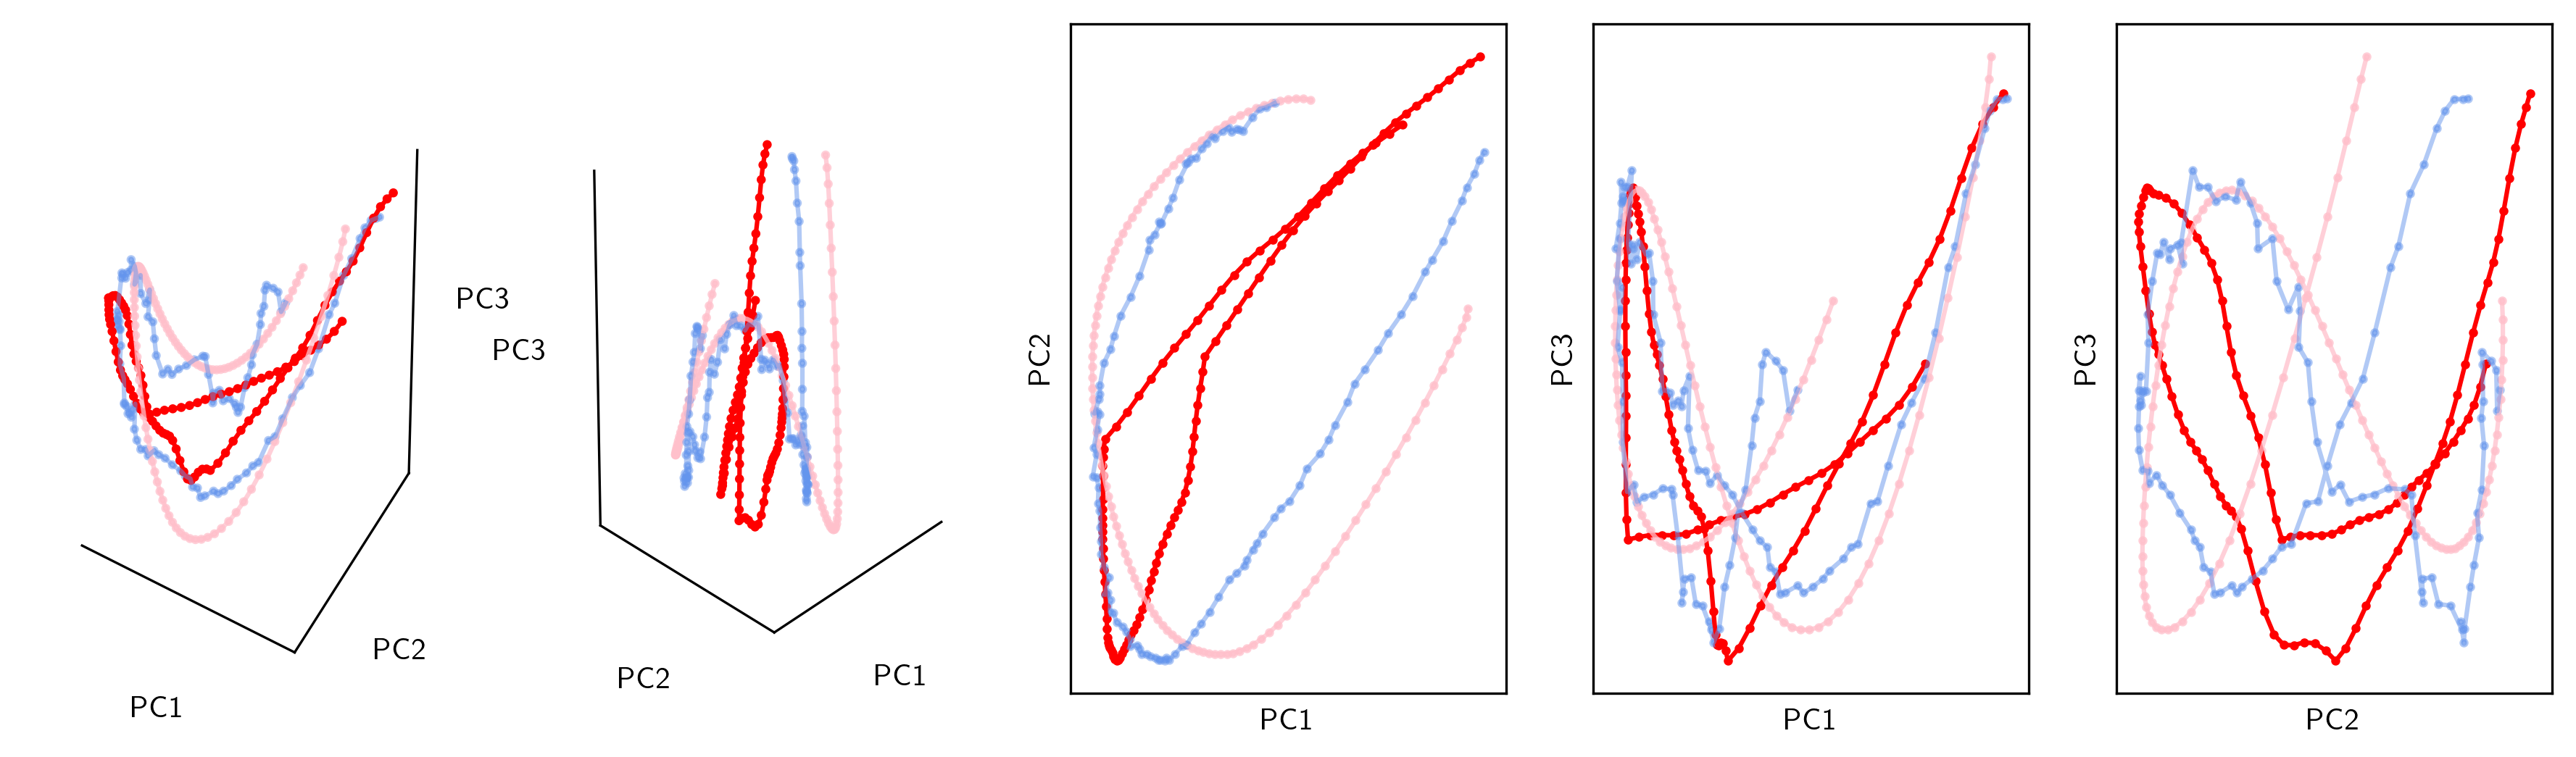
\includegraphics[width=\linewidth]{pca_noise_4.png}
    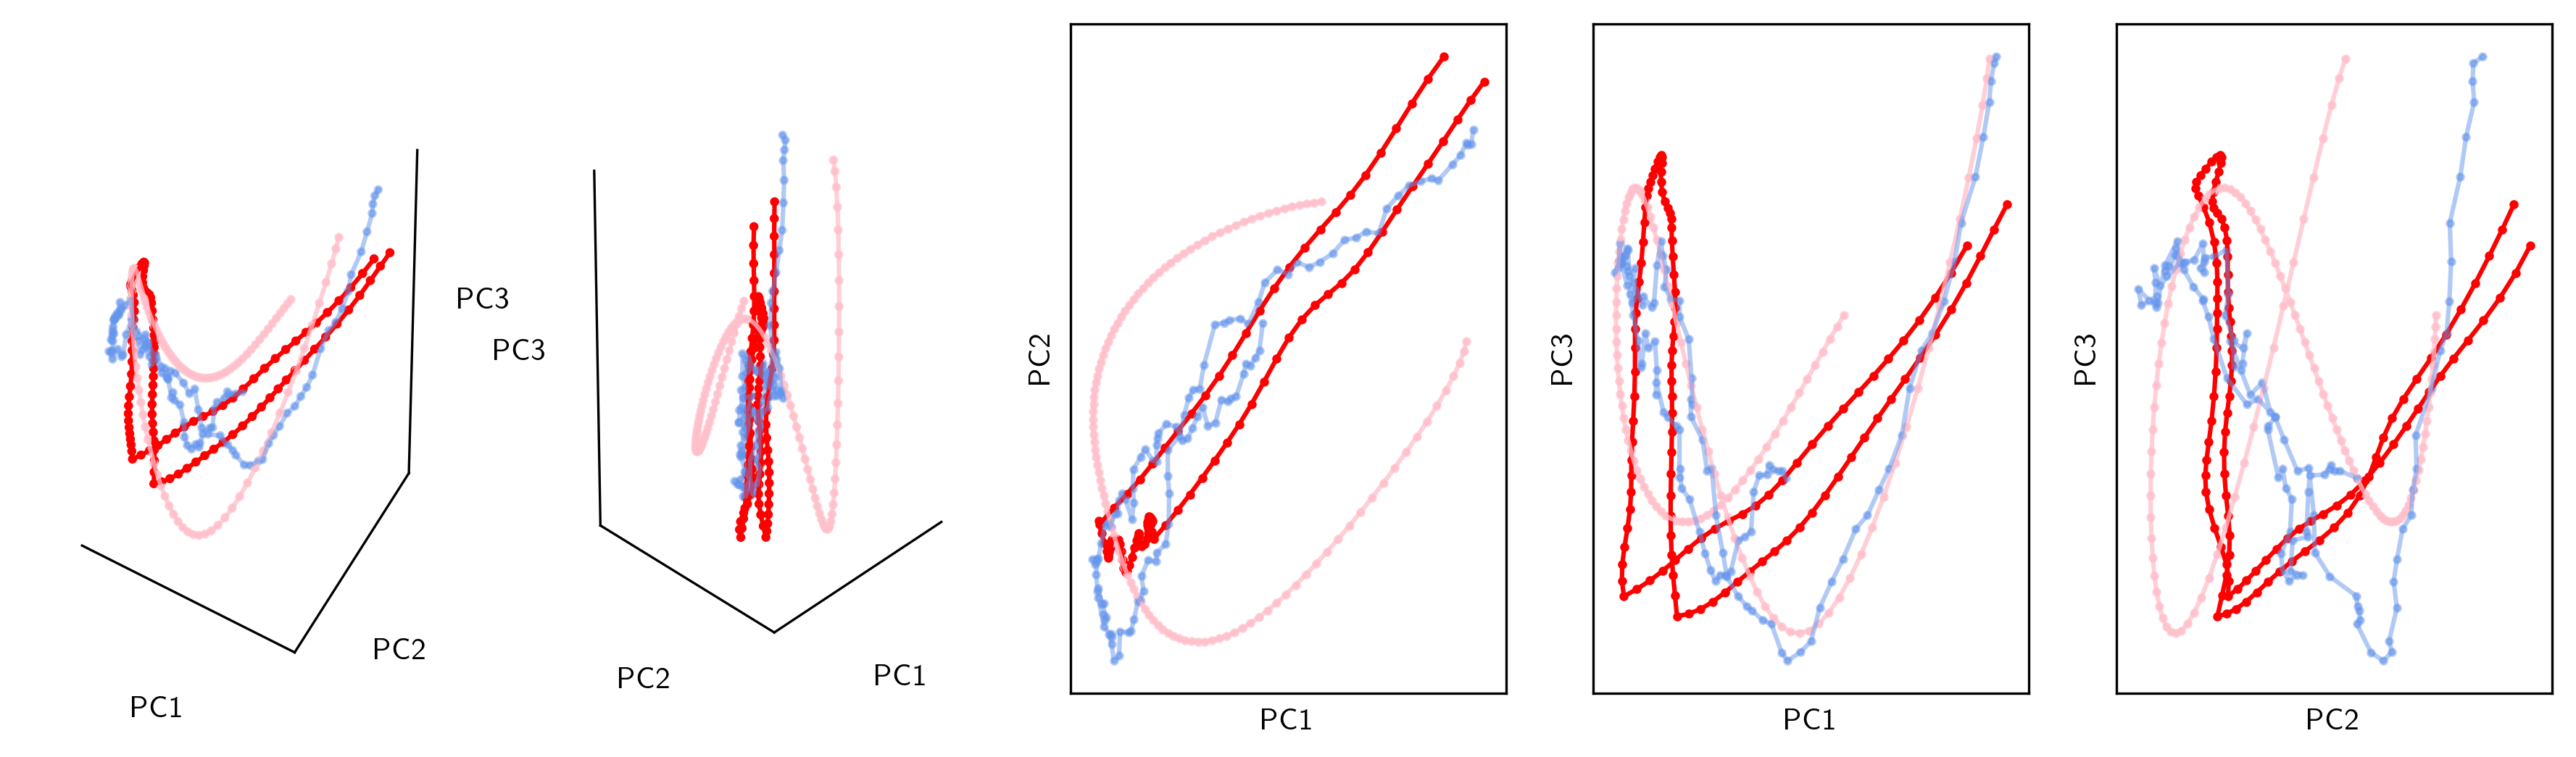
\includegraphics[width=\linewidth]{pca_noise_5.png}
    \label{fig:my_label}
\end{figure}

\begin{figure}
    \centering
    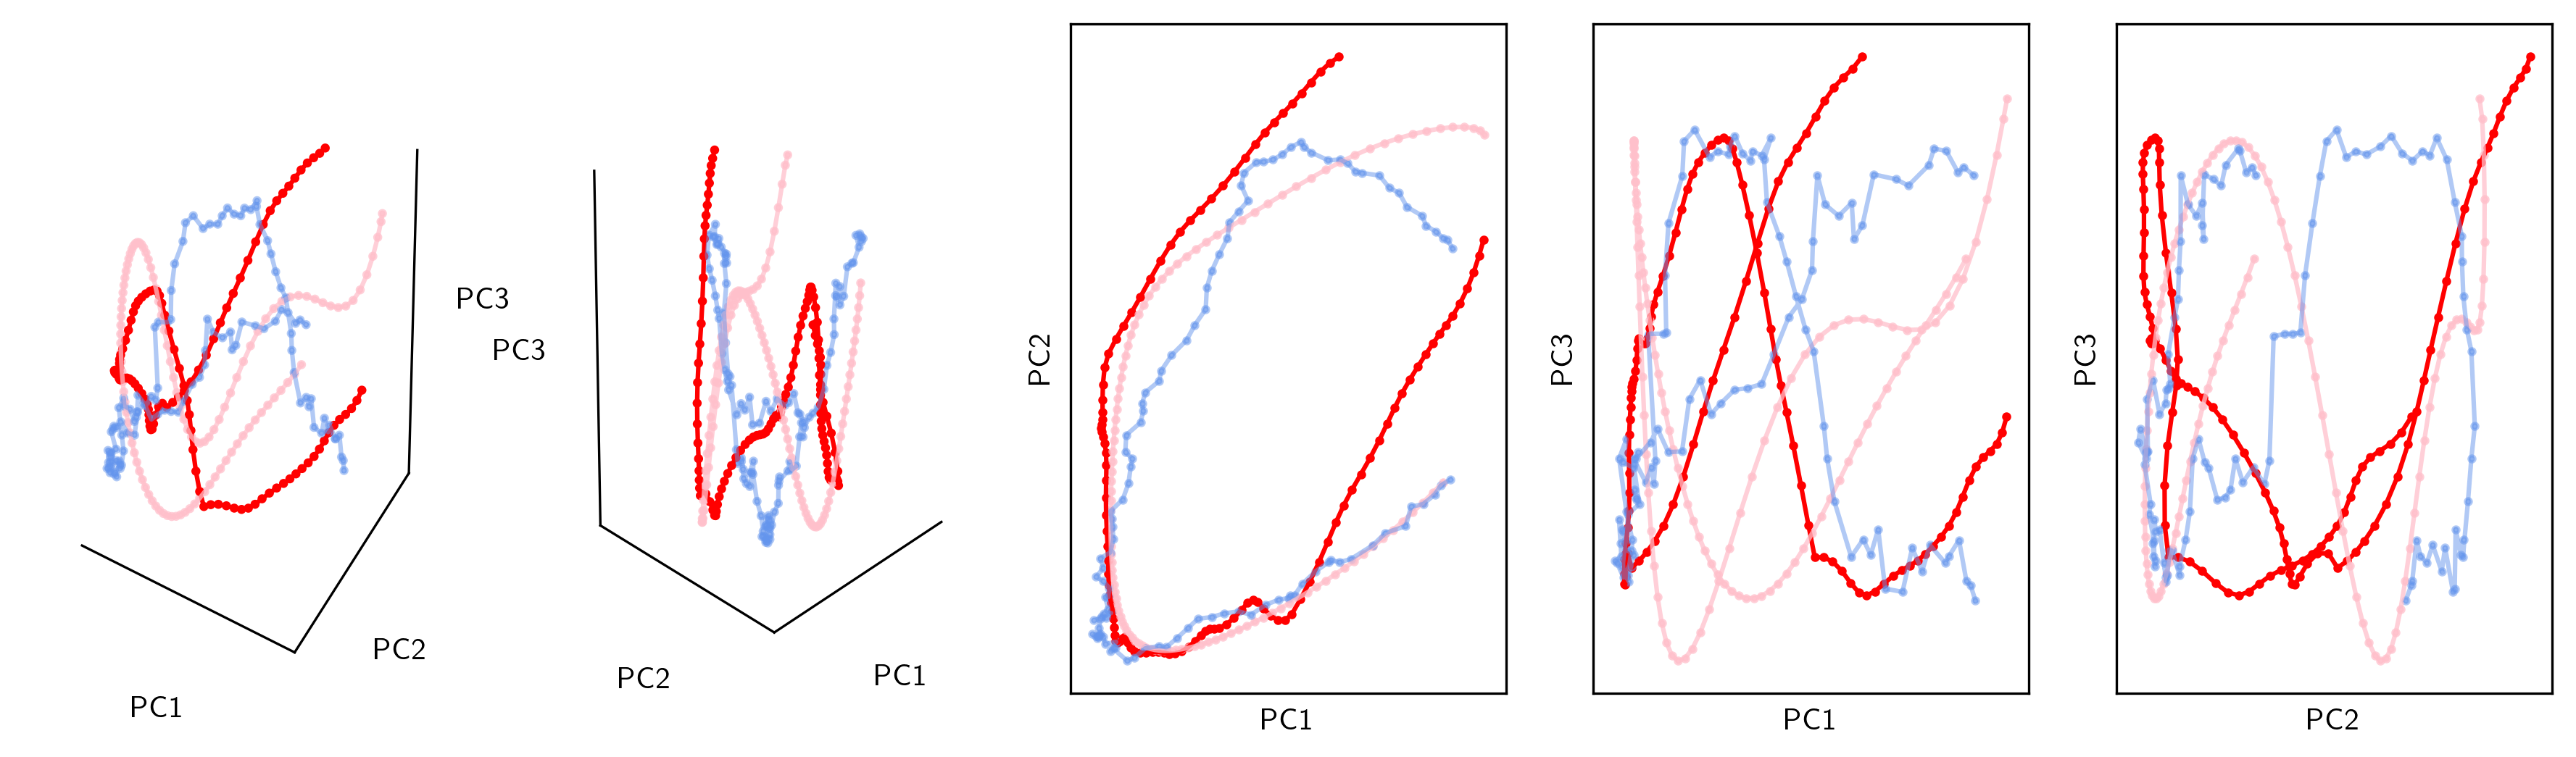
\includegraphics[width=\linewidth]{pca_noise_6.png}
    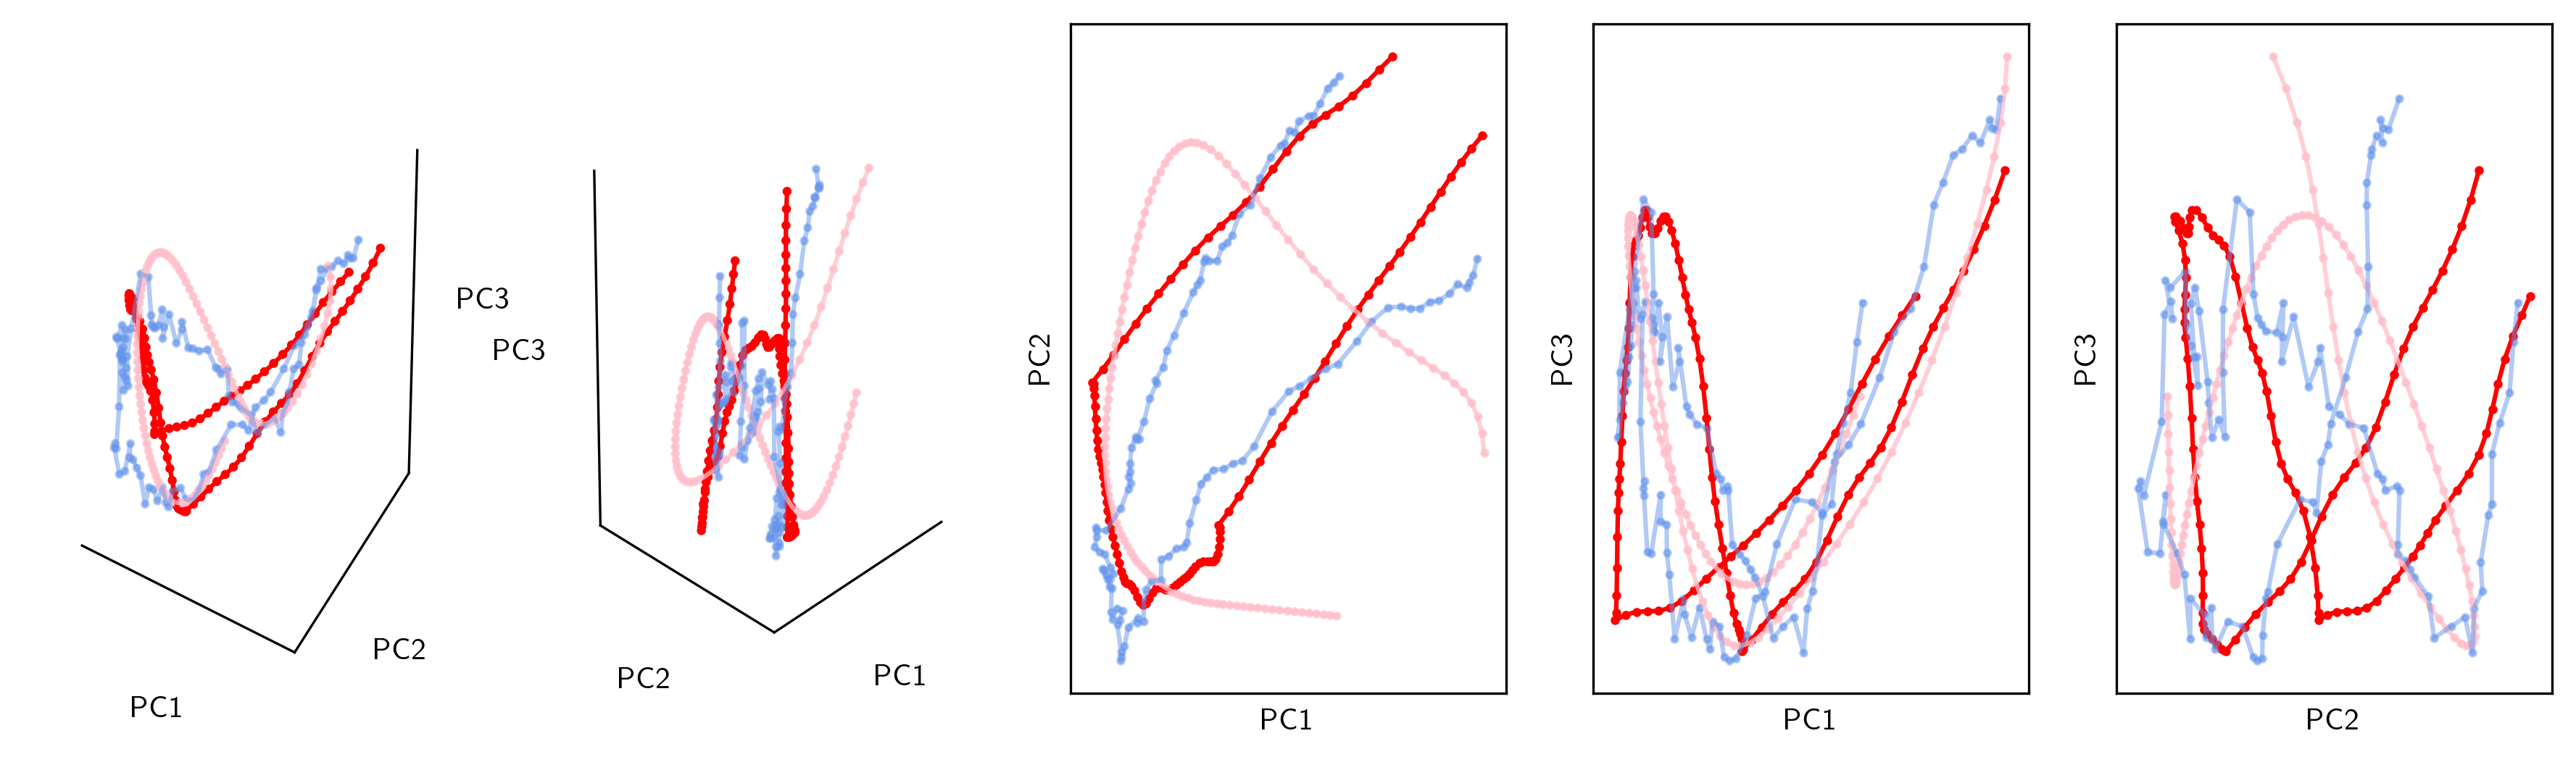
\includegraphics[width=\linewidth]{pca_noise_7.png}
    \label{fig:my_label}
\end{figure}

\newpage

\section*{Appendix C: Dot discrimination task}
We describe the motion/color discrimination task in more detail than can be provided in the brief summary in the main section of the paper. A schematic is provided to aid in understanding the details of the task.

\begin{figure}[h!]
  \centering
  \includegraphics[width=0.85\linewidth]{monkey_fig.png}
  \caption{A schematic of the dot discrimination task, taken from \cite{Mante2013}. This shows each phase of the task, as well as the possible dot screens the monkey could have been presented with. Psychometric curves of the monkey's performance in each potential permutation of coherence between motion and color and context per trial are shown, as well.}
\end{figure}

At onset, the monkey is presented with a context cue, which indicates, in the oncoming dot display, what feature (motion or color) the monkey will have to attend to, as well as a red dot and a green dot on opposite sides of the display. Then, a noisy dot display appears that has some motion coherence of the dots moving either left or right with varying strengths between different trials, and some color coherence wherein a majority of the dots are either red or green, with the size of majority varying between trials. After some delay, the monkey is trained to perform a saccade towards the target point on the display. If the context cue indicates that the monkey must pay attention to motion, that target point is to whatever side of the dot display the dots were drifting towards. If the context cue indicates that the monkey must pay attention to color, then the monkey looks at whichever dot on the display was the majority color. In the task setup formed by Mante and Sussillo, the monkey goes through several hundred trials in one sitting, and a recording electrode is placed in the same spot in FEF for each trial. These responses were all pooled into one file, termed a "unit" by the researchers. This was done for two monkeys: A and F, although we only analyzed the neural data from monkey A.

In \hyperref[sec:back]{Background and Related Work}, we describe the scheme Mante et al. proposed, although we sacrifice detail in order to present our own findings. We provide a figure from \cite{Mante2013} to illustrate. After onset of the dot display, we see neural population spike trajectories (this is the activity of the top 12 principal components of an otherwise immensely high-dimensional system, projected onto 3 dimensions) are perturbed from rest along a feature/choice axis towards a terminal point, which can be thought of as the end of the trail where the monkey performs a saccade to report its choice.

\begin{figure}[h!]
  \centering
  \includegraphics[width=0.85\linewidth]{ss.png}
  \caption{Projections of population spike data gathered when monkeys from Mante et al.'s study performed the dot discrimination task.}
\end{figure}

What was important for Mante et al.'s eventual claims about the nature of PFC feature integration was that, as we can see in a/c and d/f, despite the fact that some complementary feature is irrelevant in a context, the neural trajectories over the state space look fairly similar (and, if not similar, at least suggest that there is activity corresponding to the irrelevant sensory stream). This would eventually lead Mante et al., to train an RNN to perform the task and back-extrapolate a selection vector mechanism, described in \hyperref[sec:back]{Background and Related Work}. 

%%%%%%%%%%%%%%%%%%%%%%%%%%%%%%%%%%%%%%%%%%%%%%%%%%%%%%%%%%%%%%%%
%%%%%%%%%%%%%%%%%%%%%%%%%%%%%%%%%%%%%%%%%%%%%%%%%%%%%%%%%%%%%%%%
%%%%%%%%%%%%%%%%%%%%%%%%%%%%%%%%%%%%%%%%%%%%%%%%%%%%%%%%%%%%%%%%
%%%%%%%%%%%%%%%%%%%%%%%%%%%%%%%%%%%%%%%%%%%%%%%%%%%%%%%%%%%%%%%%
%%%%%%%%%%%%%%%%%%%%%%%%%%%%%%%%%%%%%%%%%%%%%%%%%%%%%%%%%%%%%%%%
%%%%%%%%%%%%%%%%%%%%%%%%%%%%%%%%%%%%%%%%%%%%%%%%%%%%%%%%%%%%%%%%

\end{document}

